\documentclass[12pt, a4paper]{book}
\usepackage{amssymb}
\usepackage{amsmath}
\usepackage{amssymb}
\usepackage{amsthm}
\usepackage{fancyhdr}
\pagestyle{fancy}
\usepackage{calc}
\fancyheadoffset[LE,RO]{\marginparsep+\marginparwidth}
\fancyhfoffset[L]{0.01cm}
\fancyhfoffset[R]{0.01cm}
\renewcommand{\chaptermark}[1]{\markboth{#1}{}}
\renewcommand{\sectionmark}[1]{\markright{\thesection\ #1}}
\fancyhf{}
\fancyhead[LE,RO]{\thepage}
\fancyhead[LO]{\rightmark}
\fancyhead[RE]{\leftmark}
\fancypagestyle{plain}%
\fancyhead{} % get rid of headers
\renewcommand{\headrulewidth}{0pt} % and the line
\usepackage{titlesec} 
\usepackage{bbm}
\usepackage{mathrsfs}
\usepackage{xypic}
\usepackage{enumitem}
\setenumerate{label={\rm (\alph{*})}}
\usepackage[colorlinks=true,linkcolor=blue,urlcolor=blue]{hyperref}
\usepackage{graphicx}
\usepackage{geometry}
\geometry{a4paper,left=35mm,right=35mm, top=40mm, bottom=30mm} 
\titleformat{\chapter}[display]
{\bfseries\Large}
{\filright\MakeUppercase{\chaptertitlename} \Huge\thechapter}
{1ex}
{\titlerule\vspace{1ex}\filleft}
[\vspace{1ex}\titlerule]
\renewcommand{\thesection}{\thechapter.\arabic{section}}
\titleformat{\section}{\bfseries\large}{\thesection.}{0.3em}{}
\titlespacing{\section}{0pt}{12pt}{6pt}
\titleformat{\subsection}[runin]{\bfseries}{\thesubsection.}{0.2em}{}
\titlespacing{\subsection}{0pt}{12pt}{6pt}
\numberwithin{equation}{section}
\usepackage{etoolbox}
\makeatletter
\patchcmd{\@thm}{\thm@headfont{\scshape}}{\thm@headfont{\bfseries}}{}{}
\patchcmd{\@thm}{\thm@notefont{\fontseries\mddefault\upshape}}{}{}{}
\makeatother
\newtheorem{theorem}{Theorem}[chapter]
\newtheorem{lemma}[theorem]{Lemma}
\newtheorem*{lemmazorn}{Zorn's Lemma}
\newtheorem{proposition}[theorem]{Proposition}
\newtheorem{remo}[theorem]{Remark}
\newtheorem{corollary}[theorem]{Corollary}
\newtheorem{convention}[theorem]{Convention}
\newtheorem{counterexample}[theorem]{Counterexample}
\newtheorem{hypothesis}[theorem]{Hypothesis}
\newtheorem{question}[theorem]{Question}
\newtheorem{proposition and definition}[theorem]{Proposition and Definition}
\newtheorem{definition}[theorem]{Definition}
\newtheorem{notation}[theorem]{Notation}
\newtheorem{assumption}[theorem]{Assumption}
\newtheorem{Remark}[theorem]{Remark}
\newtheorem{remark}[theorem]{Remark}
\newtheorem{example}[theorem]{Example}
\newtheorem{conjecture}[theorem]{Conjecture}
\numberwithin{equation}{section}
\renewcommand{\baselinestretch}{1.2}\normalsize
\providecommand{\meantmp}[2]{#1\langle{#2}#1\rangle}
\providecommand{\mean}[1]{\meantmp{}{#1}}
\providecommand{\bigmean}[1]{\meantmp{\big}{#1}}
\providecommand{\Bigmean}[1]{\meantmp{\Big}{#1}}
\providecommand{\biggmean}[1]{\meantmp{\bigg}{#1}}
\providecommand{\Biggmean}[1]{\meantmp{\Bigg}{#1}}
\providecommand{\Ma}{\ensuremath{\mathcal{M}^\alpha}}
\providecommand{\Mas}{\ensuremath{\mathcal{M}^\alpha_\sigma}}
\providecommand{\Na}{\ensuremath{\mathcal{N}^{\alpha}}}
\providecommand{\Nares}{\ensuremath{\Na_{\text{res}}}}
\providecommand{\comment}[1]{\vskip.3cm
\fbox{%
\parbox{0.93\linewidth}{\footnotesize #1}}
\vskip.3cm}
\def\Xint#1{\mathchoice
{\XXint\displaystyle\textstyle{#1}}%
{\XXint\textstyle\scriptstyle{#1}}%
{\XXint\scriptstyle\scriptscriptstyle{#1}}%
{\XXint\scriptscriptstyle\scriptscriptstyle{#1}}%
\!\int}
\def\XXint#1#2#3{{\setbox0=\hbox{$#1{#2#3}{\int}$ }
\vcenter{\hbox{$#2#3$ }}\kern-.6\wd0}}
\def\ddashint{\Xint=}
\def\dashint{\Xint-}
\newcommand{\id}{\operatorname{Id}}
\newcommand{\diag}{\operatorname{diag}}
\newcommand{\diam}{\operatorname{diam}}
\newcommand{\cof}{\operatorname{cof}}
\newcommand{\im}{\operatorname{im}}
\newcommand{\bd}{\operatorname{BD}}
\newcommand{\bv}{\operatorname{BV}}
\newcommand{\BV}{\operatorname{BV}}
\newcommand{\BD}{\operatorname{BD}}
\newcommand{\Leb}{\mathbf{L}}
\newcommand{\sbd}{\mathbf{SBD}}
\newcommand{\bdiv}{\mathbf{BD}_{\text{div}}}
\newcommand{\bviv}{\mathbf{BV}_{div}}
\newcommand{\ld}{\operatorname{LD}}
\newcommand{\ep}{\varepsilon}
\newcommand{\di}{\operatorname{div}}
\newcommand{\Lip}{\operatorname{Lip}}
\newcommand{\essential}{\operatorname{esssup}}
\newcommand{\dif}{\operatorname{d}}
\newcommand{\Radonfin}{M_{b}(\Omega,\mathbb{R}_{\text{sym}}^{d\times d})}
\newcommand{\Radon}{M_{b}(\Omega,\mathbb{R}^{d\times d})}
\newcommand{\DIF}{\mathbf{D}}
\newcommand{\spt}{\operatorname{spt}}
\newcommand{\N}{\mathbb{N}}
\newcommand{\X}{\mathbf{X}}
\newcommand{\tr}{\operatorname{tr}}
\newcommand{\eind}{\operatorname{ell ind}}
\newcommand{\cod}{\operatorname{codim}}
\newcommand{\cok}{\operatorname{Coker}}
\newcommand{\R}{\mathbb{R}}
\newcommand{\x}{\mathbf{x}}
\newcommand{\uu}{\mathbf{u}}
\newcommand{\meas}{\operatorname{meas}}
\newcommand{\locc}{\operatorname{loc}}
\newcommand{\sing}{\operatorname{Sing}}
\newcommand{\reg}{\operatorname{Reg}}
\newcommand{\excess}{\operatorname{Ex}}
\newcommand{\brz}{\operatorname{B}(z,r)}
\newcommand{\brx}{\operatorname{B}(x,r)}
\newcommand{\brxo}{\operatorname{B}(x_{0},r)}
\newcommand{\broz}{\operatorname{B}(Z,\rho)}
\newcommand{\dist}{\operatorname{dist}}
\newcommand{\supp}{\operatorname{supp}}
\newcommand{\gp}{\mathbf{g}_{p}}
\newcommand{\range}{\operatorname{Ran}}
\newcommand{\iu}{\operatorname{i}}
\newcommand{\trace}{\operatorname{Tr}}
\newcommand{\diameter}{\operatorname{diam}}
\newcommand{\capa}{\operatorname{Cap}}
\newcommand{\ranka}{\operatorname{rank}}
\newcommand{\ranga}{\operatorname{Ran}}
\newcommand{\bvc}{\operatorname{BV}_{\operatorname{c}}}
\newcommand{\E}{\mathbf{E}}
\newcommand{\wlim}{\operatorname{w^{*}-}\lim_{\varepsilon\searrow 0}}
\newcommand{\wstar}{\stackrel{*}{\rightharpoonup}}
\newcommand{\ball}{\operatorname{B}}
\renewcommand{\rho}{\varrho}
\newcommand{\Cc}{\operatorname{C}_{\operatorname{c}}}
\renewcommand{\c}{\operatorname{c}}
\renewcommand{\hom}{\operatorname{Hom}}
\newcommand{\W}{\operatorname{W}}
\newcommand{\ellind}{\operatorname{ellind}}
\newcommand{\spano}{\operatorname{span}}
\newcommand{\Con}{\operatorname{C}}
\newcommand{\ad}{\mathbb{A}[D]u}
\newcommand{\gm}{\operatorname{GM}}
\newcommand{\finfty}{f^{\infty}}
\newcommand{\yhat}{\ensuremath{\hat{y}}}
\newcommand{\bspq}{\operatorname{B}_{p,q}^{s}}
\newcommand{\lpw}{\operatorname{L}_{\omega}^{p}}
\newcommand{\lp}{\operatorname{L}^{p}}
\newcommand{\lloc}{\operatorname{L}_{\operatorname{loc}}^{1}}
\newcommand{\mes}{\operatorname{mes}}
\newcommand{\lebe}{\operatorname{L}}
\newcommand{\sobo}{\operatorname{W}}
\newcommand{\besov}{\operatorname{B}}
\newcommand{\pv}{\operatorname{pv}}
\newcommand{\hold}{\operatorname{C}}
\newcommand{\traceop}{\operatorname{Tr}}
\newcommand{\bvloc}{\operatorname{BV}_{\operatorname{loc}}}
\renewcommand{\epsilon}{\varepsilon}
\newcommand{\lpnorm}{\|\cdot\|_{p,\Omega}}
\newcommand{\Span}{\operatorname{span}}
\newcommand{\aff}{\operatorname{aff}}
\newcommand{\con}{\operatorname{conv}}
\newcommand{\B}{\mathbb B}
\newcommand{\rank}{\operatorname{rank}}
\newcommand{\interior}{\operatorname{int}}
\newcommand{\Le}{\mathscr{L}^{n}}
\newcommand{\so}{\operatorname{SO}}
\newcommand{\Div}{\operatorname{div}}
\newcommand{\orth}{\operatorname{O}}
\newcommand{\spa}{\operatorname{span}}
\newcommand{\proj}{\operatorname{proj}}
\newcommand{\conv}{\operatorname{conv}}
\newcommand\myeq{\mathrel{\overset{\makebox[0pt]{\mbox{\normalfont\tiny\sffamily DCT}}}{=}}}
\newcommand\myeqIP{\mathrel{\overset{\makebox[0pt]{\mbox{\normalfont\tiny\sffamily IP}}}{=}}}
\usepackage{tikz-cd}
\begin{document}
\frontmatter
\begin{titlepage}
\begin{center}
\textsc{\LARGE University of Oxford}\\[1.5cm]

\includegraphics[width=0.25\textwidth]{ox}\\[1cm]
\textsc{\Large OxPDE Summer Project 2016}\\[0.5cm]
\newcommand{\HRule}{\rule{\linewidth}{0.5mm}}
\HRule \\[0.4cm]
{ \huge \bfseries Orthogonal Projections in Hilbert Spaces}\\[0.4cm]
\HRule \\[1.5cm]
\textsc{\Large Aili SHAO} \\
\textsc{\Large Magdalen College}
\vfill
\begin{center} {\large
\emph{Under the Supervision of}}\\
\end{center}
\begin{center}{\large 
Dr. David \textsc{Seifert}}
\end{center}
% bottom of page:
%{\large Version of \today}
\end{center}
\end{titlepage}
\newpage
\chapter{Abstract}\label{chapt:abstract}
This project is about the application of orthogonal projections in solving Poisson's equation on composite domains by using an iterative approach which is called \emph{Schwarz Alternating Method}. This classic alternating method is both discussed theoretically and numerically in this paper. The theoretical part consists of the proof of the convergence and the rate of convergence of this method, while the numerical section involves the implementation of the alogrithm in Matlab to test some theoretical conjectures.
\chapter{Acknowledgement}\label{chapt:acknowledgement}
I would like to express my special thanks to my supervisor, Dr. David Seifert, whose support throughout this project has been invaluable, particularly his constructive suggestions concerning both the mathematical proofs and the Matlab code.
\tableofcontents 
\newpage
\mainmatter
\chapter{Introduction}\label{chapt:intro}

The present work is concerned with the application of the iterated product of orthogonal projections in Hilbert space in the form of \emph{Schwarz Alternating Method}.

Consider the following Neumann problem on a 
composite domain $\Omega=\Omega_1\cup\Omega_2$ where $\Omega\subset \mathbb{R}^n$ is open and bounded.
$$\begin{cases}
-\Delta u+u=f \mbox{ in } \Omega,\\
\frac{\partial u}{\partial n}=0 \mbox{ on } \partial\Omega.\\
\end{cases}$$ 

One iterative approach for solving the above Neumann problem is the classic \emph{Schwarz Alternating Method}, which forms the starting point for \emph{domain decomposition techniques}. Our aim in this paper is to first introduce the \emph{Schwarz Alternating Method} mathematically, and then implement the algorithm for the two-dimensional composite domain in Matlab.

The organisation of this paper is as follows:

Chapter \ref{chapt:Iterated_Products_of_Projections_in_Hilbert_Space}
introduces the theorem on convergence of the iterated products of an arbitrary finite number of orthogonal projections in Hilbert space which is known as the \emph{von-Neumann Halperin Theorem}.

In chapter \ref{chapt:rate of convergence}, we follow the 2015 paper of \emph{Deutsch} and \emph{Hundal}\cite{DH15}, which introduces the \emph{Dichotomy Theorem} concerning the rate of convergence of the iterated products of linear operators and its applications in cyclic projections. We also introduce the concept of \emph{Friedrichs Angles} to present the rate of convergence for the two-dimensioanl case in a more elegant way.

First two sections of chapter \ref{chapt:SAM} follow the 1988 paper of \emph{P.L.LIONS}\cite{PL88}, which introduces the \emph{Schwarz Alternating Method} that we use to describe the algorithm for solving the Neumann problem in both one-dimensional and two-dimensional composite domains. We then implement the algorithm in Matlab to solve the Poisson's equation with Neumann boundary condtions in a specific L-shaped domain and demonstrate the rate of convergence by plotting the error norms against the number of iterations.



\chapter{Iterated Products of Orthogonal Projections in Hilbert Space}\label{chapt:Iterated_Products_of_Projections_in_Hilbert_Space}In this chapter, we focus on the convergence of the iterated products of orthogonal projections in Hilbert Space. This classical result was first estabilished for two orthogonal projections by \emph{J.Von Neumann}\cite{JN33} in 1933 in the form of the following theorem:
\begin{theorem}
Let $X$ be a Hilbert Space, and $M_1,M_2$ be closed subspaces of $X$. If $P_{M_i}$ is an orthogonal proection on $M_i$ for eacu $i=1,2$, and $P_{M}$ is the orthogonal projection on the closed subspace $M=M_1\cap M_2$, then for each $x\in X$,
$$\lim_{n\rightarrow\infty}(P_{M_1}P_{M_2})^n(x)=P_{M}(x).$$
\end{theorem}

We can simply demonstrate this beautiful result in the two-dimensional case:

Let $M_1$ and $M_2$ be the two straight lines as shown in the diagram below, and $x$ be an arbitrary element from $\mathbb{R}^2$. If we define an alternating sequences $\{x_n\}$ by
$$x_0=x,$$
$$x_{2n+1}=P_{M_1}(x_{2n}),$$
$$x_{2n}=P_{M_2}(x_{2n-1})=(P_{M_1}P_{M_2})^n(x_0)), $$
then $\lim_{n\rightarrow\infty}x_n=P_{M}(x).$
\begin{figure}[h]
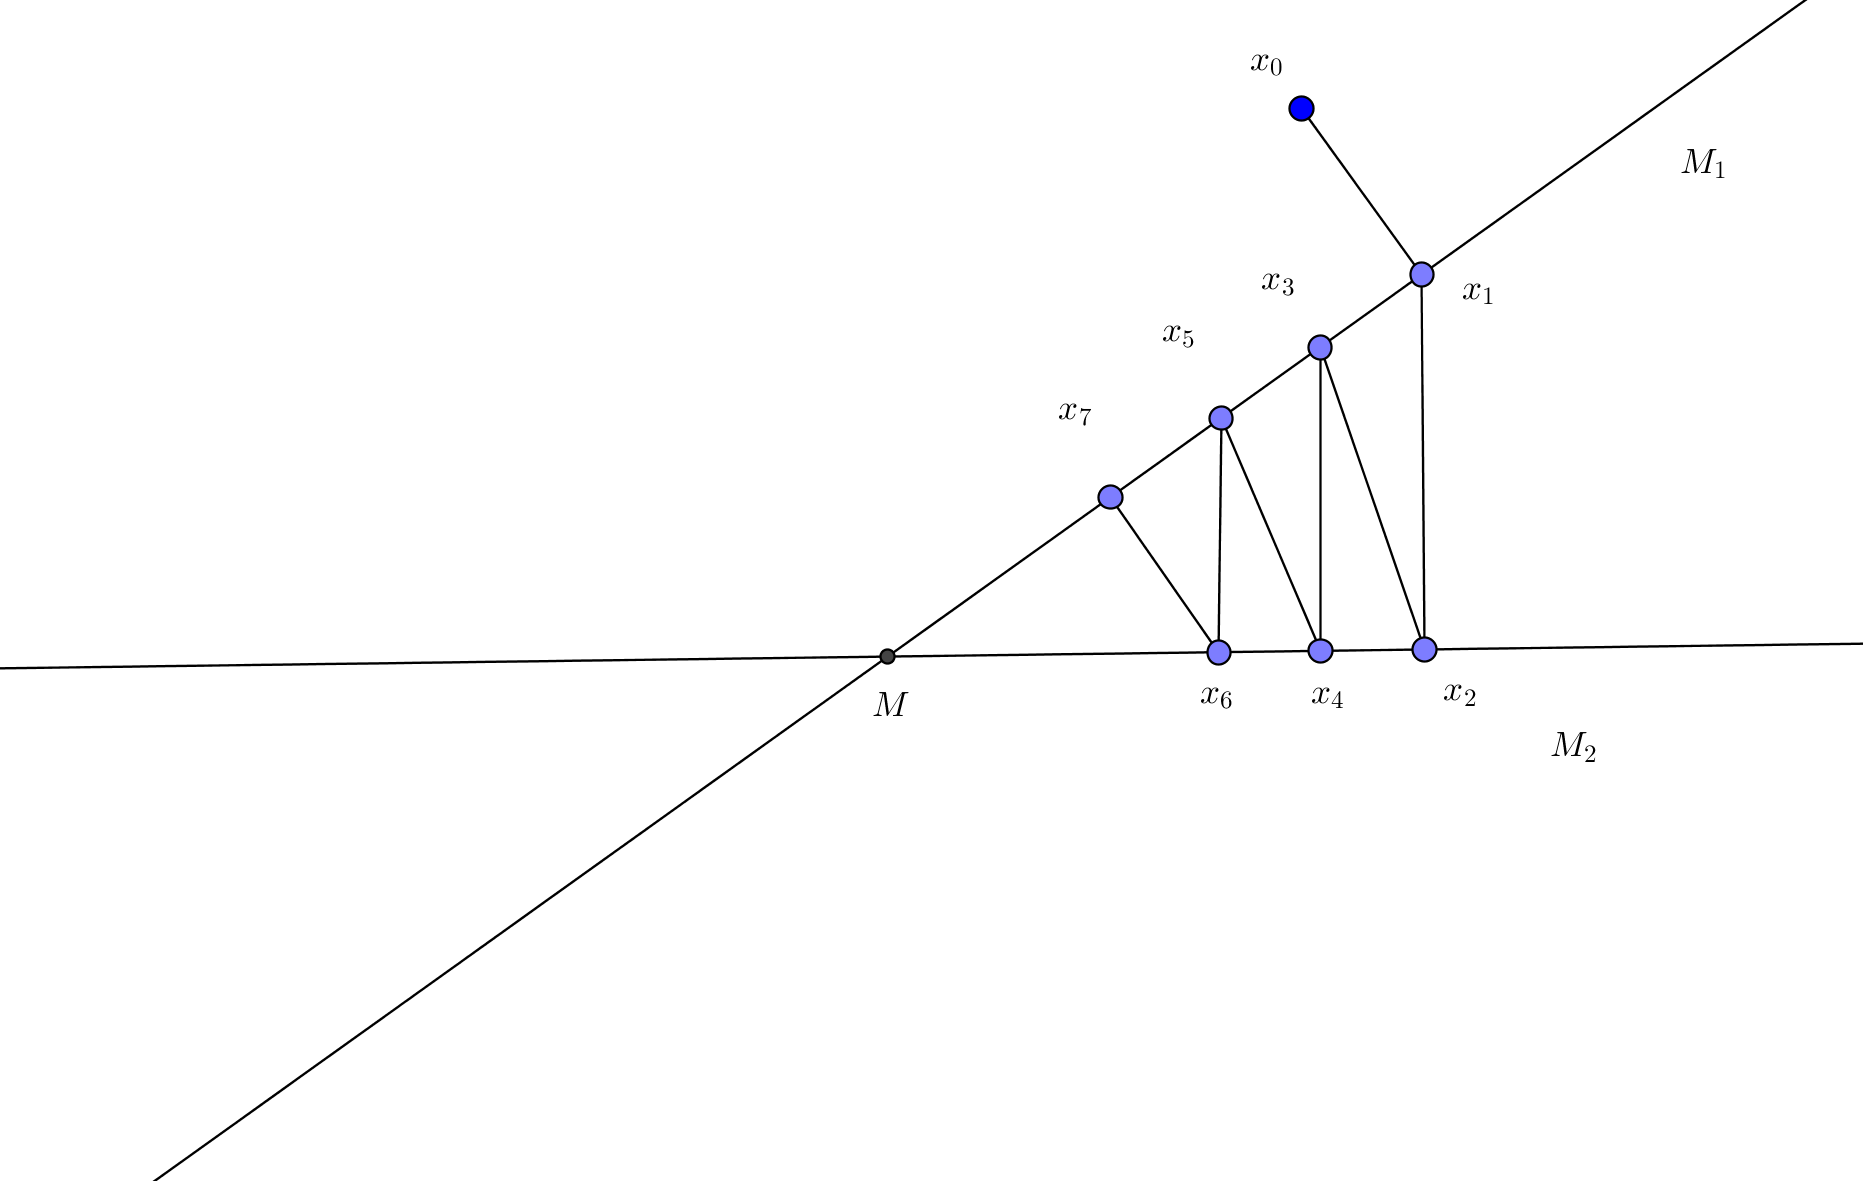
\includegraphics[width=140mm,scale=0.8]
{2d_demo.png}
\end{figure}
\par
 The same theorem was also found by \emph{Nakano} \cite{NN53} in 1953 and \emph{Wiener}\cite{NW55} in 1955. Indeed, the result is also true for any arbitrary finite number of orthogonal projections as shown in \emph{Halperin's} work \cite{IH62} in 1962.

\section{Convergence of the Iterated Products of Orthogonal Projections}
In this section, we present a detailed proof of Halperin's result based on \emph{Kakutani's} lemma and proof \cite{SK40}.
\begin{theorem}[von-Neumann Halperin]\label{halperin}Let $X$ be a Hilbert space and $P_j$ be the orthogonal projection onto the closed subspace $M_j$ of the Hilbert space $X$ for each $1\leq j\leq k$. Let $P_{M}$ be the orthogonal projection onto the intersection $M=M_1\cap M_2\cdots \cap M_k$. If $T=P_k\cdots P_1$, then $\|T^n x-P_{M}x\|\rightarrow 0$ for each $x\in X$ as $n\rightarrow\infty.$
\end{theorem}
Before we proceed to the proof of the main theorem, we introduce \emph{Kakutani's} lemma first:
\begin{lemma}[Kakutani's Lemma]\label{1}
Let $P_j$ and $T$ be defined as above. Then $\|T^n x-T^{n+1}x\|\rightarrow 0$ as $n\rightarrow\infty$.
\begin{proof}
For any $x\in X$, we have $$\|T^{n+1}x\|\leq \|T\|\|T^{n}x\|\leq \|P_k\|\cdots \|P_1\|\|T^n x\|\leq \|T^n x\|,$$ This shows that $\{\|T^n x\|\}$ is a decreasing sequence in $\mathbb{R}$ that is bounded below, thus it converges. In particular, $$\|T^n x\|^2-\|T^{n+1} x\|^2\rightarrow 0$$ as $n\rightarrow \infty$. Recall the Pythagorean Theorem which gives for any orthogonal projection $P$ and any $x\in X$,$$\|x-Px\|^2=\|x\|^2-\|Px\|^2.$$
Define $Q_0=I$ and for $j=1,2,\cdots k, Q_j=P_jQ_{j-1}$, so that $Q_k=T$, then
\begin{align*}
\|T^n x-T^{n+1}x\|^2&=\|\sum_{j=0}^{k-1}(Q_jT^n x-Q_{j+1}T^n x\|^2\\
&\leq \{\sum_{j=0}^{k-1}\|(Q_jT^n x-Q_{j+1}T^n x\|\}^2 \mbox{(By triangle inequality)}\\
&\leq \left(\sum_{j=0}^{k-1}1 \right) \left( \sum_{j=0}^{k-1} \|(Q_j T^n x-Q_{j+1}T^n x\|^2 \right) \mbox {(By Cauchy-Schwarz inequality)}\\
&=k\left( \sum_{j=0}^{k-1} \|(Q_j T^n x-Q_{j+1}T^n x\|^2 \right)\\
&=k\left(\sum_{j=0}^{k-1} \|(Q_j T^n x\|^2-\|Q_{j+1}T^n x\|^2 \right)\mbox{ (By Pythagorean Theorem)}\\
&=k \left(\|Q_0 T^n x\|^2-\|Q_k T^n x\|^2 \right)\\
&=k \left(\|T^n x\|^2-\|T^{n+1} x\|^2 \right)\\
&\rightarrow 0\\ 
\end{align*}
 as $\|T^n x\|^2-\|T^{n+1} x\|^2\rightarrow 0.$
\end{proof}
\end{lemma}

Now we are ready to prove Theorem \ref{halperin}.
\begin{proof}
First note that
\begin{align*}
X&=\left(\mathrm{Im}(I-T)\right)^{\perp}\oplus\left(\mathrm{Im}(I-T)\right)^{\perp\perp} \mbox{ (Projection Theorem)}\\
&=\left(\mathrm{Im}(I-T)\right)^{\perp}\oplus\overline{\mathrm{Im}(I-T)^{\perp}}\\
&=\mathrm{Ker}(I-T^{\ast})\oplus\overline{\mathrm{Im}(I-T)^{\perp}}\\
\end{align*}

By Lemma \ref{1} $\|T^n(I-T)x\|=\|T^n x-T^{n+1}x\|\rightarrow 0$ as $n\rightarrow\infty$, then $\|T^n y\|\rightarrow 0$ for $y\in Im(I-T)$. As $\|T^n\|\leq\|T\|^n\leq (\|P_k\|\cdots \|P_1\|)^n\leq 1$, $T^n$ is a bounded linear operator, then $\|T^n y\|\rightarrow 0$ for $y\in \overline{\mathrm{Im}(I-T)}$.
If we can show that
\begin{equation}\label{2}
\mathrm{Ker}(I-T^{\ast})=M_1\cap M_2\cdots \cap M_k,
\end{equation} 
then for each $x\in X$, we have $x=y+z$ such that $y\in \mathrm{Im}(I-T)$ while $z\in M$, and then
$$\|T^n x-z\|=\|T^n(y+z)-z\|\leq \|T^n y\|+\|T^n z-z\|\rightarrow 0 $$
as $n\rightarrow \infty$.
Take $z=P_M(x)$, then the theorem follows.

\par
To show (\ref{2}), it suffices to show that $T^{\ast}x=x$ if and only if $P_i x=x$ for each $1\leq i\leq k$. If $P_i x=x$ for each $1\leq i\leq k$, then $T^{\ast}x=(P_k\cdots P_1)^{\ast}=P_1^{\ast}\cdots P_k^{\ast}x=P_1P_2\cdots P_k x=x$. Conversely, if $P_ix\neq x$ for some $1\leq i\leq k$, then $\|T^{\ast}x\|=\|P_1P_2\cdots P_k x\|\leq \|P_i x\|< \|x\|$, that is, $T^{\ast}x\neq x$.
\end{proof}


 

\chapter{Rate of Convergence}\label{chapt:rate of convergence}
In the previous chapter, we have shown that for an arbitray finite number of orthogonal proections $P_{i}$ for $i=1,2,\cdots$, $T=P_{r}P_{r-1}\cdots P_{1}$, $T^n$ converges to $P_{M}$ strongly as $n\rightarrow \infty$, but we are not sure about how fast it converges. It is crucial to study the rate of convergence when the orthogonal projections are used in applications, such as the \emph{Schwarz Alternating Method}, which we will discuss in the next chapter.


In this chapter, we will give a detailed discussion about the rate of convergence. We first study the dichotomy results from \emph{Deutsch} and \emph{Hundal's} work\cite{DH15} in 2015, and give a proof for a slightly weaker result of the general Hilbert Space case. The second half of the chapter focuses more on the concept of \emph{Friedrichs Angles} which gives a good description for the particular two closed subspaces case for the method of alternating projections.
\section{Dichotomy Results}\label{sec:dichotomy results}
Here we present a dichotomy theorem which is slightly different from the one introduced by \emph{Deutsch} and \emph{Hundal}:
\begin{theorem}(\cite{DH15})\label{theorem}
Let $X$ be a Banach space and $T\colon X\to X$ be a linear operator with $\|T\|\leq 1$ and $T^n(x)\rightarrow 0$ for each $x\in X$, then exactly one of the following two statements hold:
\begin{enumerate}
\item there exists $n_1\in\mathbb{N}$ such that $\|T^{n_1}\|<1$, and there exists $\alpha\in [0,1)$ and $c\in \mathbb{R}$ such that $\|T^n\|\leq c\alpha^n$ for each $n$.
\item $\|T^n\|=1$ for each $n\in\mathbb{N}$, and for each $(r_n)\in c_0$, $r_n\in\mathbb{R}^{+}$, for all $x\in X$, $\|T^n x\|\neq O(r_n)$.
\end{enumerate}
\begin{proof}
For $T\in B(X)$, $\mathrm{r}(\sigma(T))=\lim_{n\rightarrow\infty}\|T^n\|^{\frac{1}{n}}\leq \lim_{n\rightarrow\infty}\|T\|\leq 1$. This shows that the spectrum of $T$ lie in the closed unit disc. 

If $\mathrm{r}(\sigma(T))<1$, then there exists $n_1\in\mathbb{N}$ such that $\rho:=\|T^{n_1}\|<1$.
 
If $\rho>0$, we take $\alpha:=\rho^{\frac{1}{n_1}}$, for any $n\in\mathbb{N}$, we can write $n=kn_1+i$ for some non-negative integer $k$ and $i\in\{0,1,\cdots n_{1}-1\}$. Then $\|T^n\|=\|T^{kn_1+i}\|\leq \|T^{n_1}\|^k=\rho^k=\alpha^{n_1k}\leq c\alpha^n$ where $c= \frac{1}{\alpha^{n_1-1}}$.

If $\rho=0$, $\|T^n\|\leq 2^{n_1}(\frac{1}{2})^n$ for each $n\in\mathbb{N}$, then we take $\alpha=\frac{1}{2}$ and $c=2^{n_1}$.
\par
If $\mathrm{r}(\sigma(T))=1$, then $\mathrm{r}(\sigma(T))\leq\|T\|\leq 1$ implies $\|T\|=1$. $\|T^n\|=1$ for each $n\in\mathbb{N}$ since if $\|T^N\|<1$ for some $N\in\mathbb{N}$, we have $\mathrm{r}(\sigma(T))=lim_{n\rightarrow \infty}\|T^n\|^{\frac{1}{n}}\leq\lim_{n\rightarrow \infty}\|T^N\|^{\frac{1}{n}}<1$ which yields a contradiction. We assume for contradiction that for each $x\in X$, there exists constant $c_x>0$ such that $\|T^n x\|\leq c_x r_n$ for each $n\in\mathbb{N}$. Since $X$ is a Banach Space, \emph{Uniform Boundedness Theorem} tells $\|T^n\|\leq C r_n$ with $C$ independent of $x$, then $\|T^n\|\rightarrow 0$ as $n\rightarrow \infty$. This contradicts $\|T^n\|=1$. 
\end{proof}
\end{theorem}

Before applying the above dichotomy results to the rate of convergence of the cyclic projections in Hilbert space, we first introduce an important lemma which was proved by \emph{Bauschke, Borwein and Lewis} in \cite{BL97} by using regularities:
\begin{lemma}\label{lemma}
Let $M_i$ for $1\leq i\leq r$ be closed subspaces in the Hilbert space $X$, and $M:=\bigcap_{i}^r M_i.$ Let $P_{M_i\cap M^{\perp}}$ be the orthogonal projection onto $M_i\cap M^{\perp}$ for each $i=1,2,\cdots r$. Then the following are equivalent 
\begin{enumerate}
\item $\sum_{i=1}^r M_{i}^{\perp}$ is closed;
\item $\|P_{M_r\cap M^{\perp}}P_{M_{r-1}\cap M^{\perp}}\cdots P_{M_1\cap M^{\perp}}\|<1;$
\end{enumerate}
\end{lemma}
Now we can deduce the \emph{Von Neumann-Halperin Dichotomy} from \emph{Theorem} \ref{theorem} and the above lemma:
\begin{theorem}(\cite{DH15})\label{theorem2}
Let $M_i$ for $1\leq i\leq r$ be closed subspaces in the Hilbert space $X$, and $M:=\bigcap_{i}^r M_i.$ Let $T=P_{r}P_{r-1}\cdots P_{1}$ where $P_{i}$ is the orthogonal projection on $M_i$. Then exactly one of the two following statements holds:
\begin{enumerate}
\item $\sum_{i=1}^r M_{i}^{\perp}$ is closed, then there exists $\alpha\in [0,1)$ and $c\in \mathbb{R}$ such that $\|T^n-P_{M}\|\leq c\alpha^n$ for each $n$.
\item $\sum_{i=1}^r M_{i}^{\perp}$ is not closed, then for each $(r_n)\in c_0$, $r_n\in\mathbb{R}^{+}$, for all $x\in X$, $\|T^n x-P_{M}x\|\neq O(r_n)$.
\end{enumerate}
\begin{proof}
If $\sum_{i=1}^r M_{i}^{\perp}$ is closed, we have $\|P_{M_r\cap M^{\perp}}P_{M_{r-1}\cap M^{\perp}}\cdots P_{M_1\cap M^{\perp}}\|<1$ (by \emph{Lemma \ref{lemma}}).

Note that 
\begin{align*}
T^n-P_{M}&=T^n-T^nP_M \\
{}&=T^n(I-P_{M})\\
{}&=T^n P_{M^{\perp}}\\
{}&=T^n P_{M^{\perp}}^n \mbox{ since } P_{M^{\perp}}^2=P_{M^{\perp}}\\
{}&=(TP_{M^{\perp}})^n \mbox{ since } T \mbox{ commutes with } P_{M^{\perp}}\\
{}&=[(P_{r}P_{M^{\perp}})(P_{r-1}P_{M^{\perp}})\cdots (P_{1}P_{M^{\perp}})]^n\\
{}&=[(P_{M_r\cap M^{\perp}})(P_{M_{r-1}\cap M^{\perp}})\cdots (P_{M_1\cap M^{\perp}})]^n.
\end{align*}
The second last equality follows from $P_{i}$ commuting with $P_{M^{\perp}}$ and $P_{M^{\perp}}^2=P_{M^{\perp}}$ while the last equality is true because $P_{i}P_{M^{\perp}}=P_{M_i\cap M^{\perp}}$.

By taking $\|P_{M_r\cap M^{\perp}}P_{M_{r-1}\cap M^{\perp}}\cdots P_{M_1\cap M^{\perp}}\|=\alpha\in [0,1)$, we have 
\begin{align*}
\|T^n-P_{M}\|&=\|[(P_{M_r\cap M^{\perp}})(P_{M_{r-1}\cap M^{\perp}})\cdots (P_{M_1\cap M^{\perp}})]^n\|\\
{}&\leq \|(P_{M_r\cap M^{\perp}})(P_{M_{r-1}\cap M^{\perp}})\cdots (P_{M_1\cap M^{\perp}})\|^n\\
{}&=\alpha^n.
\end{align*}
In this case, $c=1$ and the result follows.
\par
If $\sum_{i=1}^r M_{i}^{\perp}$ is not closed, by \emph{Lemma} \ref{lemma}, $\|P_{M_r\cap M^{\perp}}P_{M_{r-1}\cap M^{\perp}}\cdots P_{M_1\cap M^{\perp}}\|=1$, and then $\|[P_{M_r\cap M^{\perp}}P_{M_{r-1}\cap M^{\perp}}\cdots P_{M_1\cap M^{\perp}}]^n\|=1$. By \emph{Theorem \ref{theorem}(b)}, the result follows.
\end{proof}
\end{theorem}
\section{Friedrichs Angles}\label{sec:friedrichs}
In order to apply the \emph{Von-Neumann Halperin Theorem} in the method of alternating projections, it is important to know the \emph{Friedrichs Angle} which is defined in the following sense:
\begin{definition}
Let $X$ be a Hilbert space, and $M_1$, $M_2$ are two closed subspaces of $X$ with intersection $M:=M_1\cap M_2$. The \emph{Friedrichs angle} between $M_1$ and $M_2$ is defined to be the angle in $[0,2\pi]$ whose cosine is given by
$$ c(M_1,M_2)=\sup\{|\left\langle x,y\right\rangle|\colon x\in M_{1}\cap M^{\perp}, \|x\|\leq 1, y\in M_2\cap M^{\perp},\|y\|\leq 1\}.$$
\end{definition}

Now we can deduce a relationship between the rate of convergence and the Friedrichs angle between the two closed subspaces $M_1$, $M_2$.
\begin{theorem}(\cite{KW88})\label{t1}
Let $X$ be a Hilbert space, and $M_1, M_2$ and $M$ be defined as above. If $P_1$ and $P_2$ are the orthogonal projections onto $M_1$ and $M_2$ respectively, and $P_M$ is the orthogonal projection onto $M$, then for each $n\in\mathbb{N}$, we have
$$\|(P_2P_1)^n-P_{M}\|=c(M_1,M_2)^{2n-1}.$$
\end{theorem}
Before proving the main theorem, we introduce some fundamental results first.
\begin{lemma}\label{l1}
Let $Q_i:=P_i(I-P_{M})$ for each $i=1,2$, then $$(P_2P_1)^n-P_M=(Q_2Q_1)^n.$$
\begin{proof}
\begin{align*}
(P_2P_1)^n-P_M &= (P_2P_1)^n-(P_2P_1)^n P_M\\
{}&=(P_2P_1)^n(I-P_M)\\
{}&=(P_2P_1)^n P_{M^{\perp}}\\
{}&=(P_2P_1)^n P_{M^{\perp}}^n  \mbox{ as } P_{M^{\perp}}^2=P_{M^{\perp}} \\
{}&= (P_2P_1 P_{M^{\perp}})^n   \mbox{ as } P_2P_1 \mbox{ commutes with } P_{M^{\perp}}\\
{}&=(P_2 P_{M^{\perp}} P_1 P_{M_{\perp}})^n\\
{}&=(Q_2Q_1)^n
\end{align*}
where the second last inequality follows from $P_i$ commuting with $P_{M^{\perp}}$.
\end{proof}
\begin{lemma}\label{l2}
If $T\in B(X)$ with $X$ being a Hilbert space is a self-adjoint linear operator, then for each $n\in\mathbb{N}\cup\{0\}$,
$$\|T^n\|=\|T\|^n.$$
\end{lemma}
\begin{proof}
Note that if $T$ is self-adjoint, we have $\|T^2\|=\|T\|^2$. (B4.2 Hilbert space lecture notes) 
Similarly, $\|T^4\|=\|T^2\|^2=\|T\|^4$. By induction, the result is true for $n=2^m$ with $m\in \mathbb{N}\cup\{0\}$.  

For any $n\in\mathbb{N}$ not in this form, we can write $n=2^m-r$ for some $m,r\in\mathbb{N}\cup\{0\}$, then 
$\|T\|^{n+r}=\|T^{n+r}\|\leq \|T^{n}\|\|T^r\|\leq\|T^n\|\|T\|^r$. This gives $\|T\|^n\leq \|T^n\|$, and thus $\|T^n\|=\|T\|^n$.
\end{proof}
\end{lemma} 
\begin{lemma}\label{l3}
$c(M_1,M_2)=\|Q_2Q_1\|=\sqrt{\|Q_1Q_2Q_1\|}$.
\end{lemma}
\begin{proof}
By definition, we have
\begin{align*}
c(M_1,M_2)&=\sup\{|\left\langle x,y\right\rangle|\colon x\in M_{1}\cap M^{\perp}, \|x\|\leq 1, y\in M_2\cap M^{\perp},\|y\|\leq 1\}\\
{}&=\sup\{|\left\langle P_{M_1\cap M^{\perp}}x, P_{M_2\cap M^{\perp}}y\right\rangle|\colon \|x\|\leq 1,\|y\|\leq 1\}\\
{}&=\sup\{|\left\langle P_{M_2\cap M^{\perp}}P_{M_1\cap M^{\perp}}x, y\right\rangle|\colon \|x\|\leq 1,\|y\|\leq 1\}\\
{}&=\|P_{M_2\cap M^{\perp}}P_{M_1\cap M^{\perp}}\|\\
{}&=\|(P_{M_2}P_{M^{\perp}})(P_{M_1}P_{M^{\perp}})\| \mbox{ as } P_{i} \mbox{ commutes with } P_{M^{\perp}} \mbox{ for } i=1,2 \\
{}&=\|Q_2Q_1\|.
\end{align*}
Also, $\|Q_2Q_1\|^2=\|(Q_2Q_1)^{\ast}Q_2Q_1\|=\|Q_1Q_2Q_2Q_1\|=\|Q_1Q_2Q_1\|$, then the second inequality follows.
\end{proof}
Now we are ready to prove Theorem \ref{t1}:
\begin{proof}
By Lemma \ref{l1}, $\|(P_2P_1)^n-P_M\|=\|(Q_2Q_1)^n\|$. Since $((Q_2Q_1)^n)^{\ast}=(Q_1Q_2)^n$, we have 
$$\|(Q_2Q_1)^n\|^2=\|(Q_1Q_2)^n(Q_2Q_1)^n\|=\|(Q_1Q_2Q_1)^{2n-1}\|.$$

As the operator $Q_1Q_2Q_1$ is self-adjoint, it follows from Lemma \ref{l2} that $$\|(Q_1Q_2Q_1)^{2n-1}\|=\|Q_1Q_2Q_1\|^{2n-1}.$$

By applying Lemma \ref{l3}, the result then follows.
\end{proof}
Therefore, $\|(P_2P_1)^n-P_M\|$ converges to $0$ expoentially fast if and only if $c(M_1,M_2)<1$.
\par

\begin{theorem}
Let $M_i$ for $1\leq i\leq r$ be closed subspaces in the Hilbert space $X$, and $M:=\bigcap_{i}^r M_i.$ Let $P_{i}$ and $P_{M}$ be the orthogonal projections onto $M_i$ and $M$ respectively. If $T=P_rP_{r-1}\cdots P_1$, then $\|T^n-P_M\|$ converges to $0$ exponetially fast if and only if $\mathrm{Im}(I-T)$ is closed.
\begin{proof}
Since $M:=\bigcap_{i}^r M_i$ is closed, $X=M\oplus M^{\perp}$. We have proved that $M=\mathrm{Ker}(I-T^{\ast})$, it follows that $M^{\perp}=\overline{\mathrm{Im}(I-T)}$. Let $	Y=\mathrm{Im}(I-T)$, and $Z=\overline{Y}$.

In the proof of the \emph{dichotomy results}, we have showed that the convergence is exponentially fast if and only if $r(S)<1$ where $S:=T\mid_{Z}=TP_{M^{\perp}}$.
Then $I-S\colon Z\to Z$ has trivial kernel since if
$(I-S)x=0$ for some $x\in Z$, we have $x=Sx=Tx$, that is, $x\in M^{\perp}\cap M=\{0\}$. 
We also have $\mathrm{Im}(I-S)=Y$. For each $y\in \mathrm{Im}(I-S)$, there exists $x\in Z$ such that 
\begin{align*}
y&=(I-S)x\\
{}&=x-Sx \\
{}&=x-TP_{M^{\perp}}x \\
{}&=x-Tx  \mbox{ as } x\in Z=M^{\perp}\\
{}&=(I-T)x. 
\end{align*}
This implies that $\mathrm{Im}(I-S)\subseteq Y$.
If $y\in Y=\mathrm{Im}(I-T)$, there exists $x\in X$ such that 
\begin{align*}
y&=P_{M^{\perp}}y \mbox{ as } y\in Y\subseteq M^{\perp}\\
{}&=P_{M^{\perp}}(I-T)x \\
{}&=P_{M^{\perp}}x-P_{M^{\perp}}Tx \\
{}&=P_{M^{\perp}}x-P_{M^{\perp}}^{2}Tx \\
{}&=P_{M^{\perp}}(I-P_{M^{\perp}}T)x\\
{}&=P_{M^{\perp}}(I-TP_{M^{\perp}})x \mbox{ as } T \mbox{ commutes with } P_{M^{\perp}} \\
{}&=P_{M^{\perp}}(I-S)x \\
{}&=(I-S)x.
\end{align*}
This shows that $Y\subseteq \mathrm{Im}(I-S)$.
So $I-S$ is a bounded bijiection from $Z$ onto $Y$. By \emph{Inverse Mapping Theorem}, $I-S$ is invertible if and only if $Y=Z$. So $1\in \sigma(S)$ if and only if $Y\neq Z$. That is $r(S)<1$ if and only if $Y=Z$.
\end{proof}
\end{theorem}
\chapter{Schwarz Alternating Method in elliptic PDEs}\label{chapt:SAM}
The Schwarz alternating method, first introduced by \emph{Hermann Schwarz}\cite{HS69} in 1869, is a classical iterative method for solving boundary value problem for harmonic functions. It described an iterative method for solving the Dirichlet problem in the union of two overlapping regions provided that the intersection was suitably well behaved.

In the 1950s, Schwarz's method was generalized in the theory of partial differential equations to an iterative method for finding the solution of a elliptic boundary value problem on a domain which is the union of two overlapping subdomains.  It solves the boundary value problem on each of the two subdomains in turn, passing the approximate solutions to the next boundary conditions. 

In the first section of this chapter, we start with decribing the \emph{Schwarz Alternating Method} for the one-dimensional Neumann boundary problem, and then calculate the relative \emph{Friedrichs Angles}. In the second section, this method is generalized to the two-dimensional case. Then we end this chapter with the demonstration of this method for an L-shape two-dimensional domain in Matlab.


\section{One Dimensional Case with Friedrichs Angles Calculated}\label{sec:one-d_case} 

Take $\Omega=(0,1)\subset\mathbb{R}$, and decompose $\Omega$ into two subdomains $\Omega_1:=(0,r)$, $\Omega_2:=(s,1)$ with $s\leq r$ such that $\Omega=\Omega_1\cup\Omega_2$.

In this section, we aim to apply the \emph{Schwarz Alternating Method} in solving the one-dimensional Neumann problem of the following form:
$$\begin{cases}
-u''+u=f  \mbox{ in } \Omega, \\
u'(0)=u'(1)=0\\
\end{cases}$$
where $\Omega=\Omega_1\cup\Omega_2$.

Note that for the one-dimensional case, the weak formulation of the solution of the above equation concides with the classical solution. In order to prove this claim, we need the \emph{Fundamental Lemma of Calculus of Variations}:
\begin{lemma}\label{FTCV}
For $f, g\in C(0,1)$ such that 
$$\int_{0}^{1} (f\varphi +g\varphi ') dx=0$$
for all $\varphi\in C_{0}^{\infty}(0,1)$, we have $g\in C^1(0,1)$ and $g'=f$.
\end{lemma}

The weak formuation of the solution is 
$$\int_{0}^1 u'\varphi '+u\varphi dx=\int_{0}^1 f \varphi dx$$ for all $\varphi\in C^{\infty}(0,1)$. Let $v\in C^1(0,1)$ be the primitive function of $u$, that is, $v(x)=\int_{0}^{x}u(s) ds$, while $\phi\in C_{0}^{\infty}(0,1)$ satisfy $\varphi=\int_{0}^{\infty} \phi(s) ds$. Note that 
$$\int_{0}^{1} u'\varphi ' dx=\left[ u \varphi '\right]_{0}^{1}-\int_{0}^{1} u\varphi'' dx=-\int_{0}^{1} u\varphi '' dx$$ for all $\varphi' \in C_{0}^{\infty}$. Since $\varphi'=\phi$, we have 
$$\int_{0}^{1} u'\phi=-\int_{0}^{1} u\phi ' dx$$.
Then 
\begin{align*}
\int_{0}^{1} f\varphi dx&=\int_{0}^{1} u'\varphi '+u \varphi dx\\
{}&=-\int_{0}^{1} u\phi' dx +\left[v \varphi\right]_{0}^{1}-\int_{0}^{1} v\phi dx \\
{}&=-\int_{0}^{1} u\phi' +v\phi dx
\end{align*}
If $F$ is the primitive function of $f$, say $F(x)=\int_{0}^{x} f(s) ds$, then 
$$\int_{0}^{1} f\varphi dx =\left[ F\varphi\right]_{0}^{1}-\int_{0}^{1} F \phi dx.$$
Rearranging gives 
$$\int_{0}^{1} (u\phi'+(v-F)\phi) dx.$$

By Lemma \ref{FTCV}, we have $u\in C^1$ and $u'=v-F$. Since $v, F\in C^1$, $u\in C^2$.
\subsection{The Schwarz Alternating Method}\label{sec:SAM}\hfill


Let $X=H^{1}(0,1)$. Since the one-dimensional Sobolev space $H^{1}(0,1)$ is embedded in the space $C([0,1])$ of continuous functions, we can identify each element of $H^{1}(0,1)$ with its corresponding representative in $C([0,1])$. Now define 
$$Y_1:=\overline{\{\phi\in C^{\infty}(0,1):\phi=0 \mbox{ in the neighbourhood of } [r,1)\}}=H_{0}^{1}(\Omega_1),$$ and
$$Y_2:=\overline{\{\phi\in C^{\infty}(0,1):\phi=0 \mbox{ in the neighbourhood of } (0,s]\}}=H_{0}^{1}(\Omega_2).$$

Fix $u_0\in X$ and find $u_1$ by first solving
$$\begin{cases}
-u_1''+u_1=f  \mbox{ in } \Omega_1, \\
u_1(r)=u_0(r),\\
u_1^{\prime}(0)=0,\\
\end{cases}$$ 
and then extend by $u_0$ from $\Omega_1$ to all of $\Omega$.
We repeat the procedure alternatingly to find $u_2,u_3,\cdots$ such that $u_{2n+1}$ (for $n\geq 0$) solves
$$\begin{cases}
-u_{2n+1}''+u_{2n+1}=f  \mbox{ in } \Omega_1, \\
u_{2n+1}(r)=u_{2n}(r),\\
u_{2n+1}^{\prime}(0)=0,\\
\end{cases}$$ 
while $u_{2n}$ (for $n\geq 1$) is a solution of 
$$\begin{cases}
-u_{2n}''+u_{2n}=f  \mbox{ in } \Omega_2, \\
u_{2n}(s)=u_{2n-1}(s),\\
u_{2n}^{\prime}(1)=0.\\
\end{cases}$$  
We may extend $u_{2n+1}$ by $u_{2n}$ and $u_{2n}$ by $u_{2n-1}$ respectively to all of $\Omega$.

Since $$-(u_1-u)''+(u_1-u)=0 \mbox{ in } \Omega_1,$$
$$\left\langle u_1-u,\phi\right\rangle_{H^1}=\int_{\Omega_1}(u_1-u)'\phi'+(u_1-u)\phi dx=\int_{\Omega_1}-(u_1-u)''\phi+(u_1-u)\phi dx=0$$ for all $\phi\in Y_1$. This shows that $u_1-u\perp Y_1$. Let $M_i=Y_{i}^{\perp}$ for $i=1,2$, then $u_1-u\in M_1$. 

If we take $w=u_1-u$, then $w$ satisfies
$$\begin{cases}
-w''+w=0 \mbox{ in } \Omega_1,\\
w'(0)=0.\\
\end{cases}$$
By solving the above second order ordinary differential equation (ODE), we have $w=C(e^x+e^{-x})$ for some constant $C$. So $M_1=\emph{span}\{e^x+e^{-x}\}$.

Similarly, $v:=u_2-u\in M_2$ and satisfies 
$$\begin{cases}
-v''+v=0 \mbox{ in } \Omega_2,\\
v'(1)=0.\\
\end{cases}$$

The above ODE is solved by $v=D(e^x+e^{2-x})$ for some constant $D$, so $M_2=\emph{span}\{e^x+e^{2-x}\}$.

Note that $u_0-u=(u_0-u_1)+(u_1-u)$ where $u_0-u_1\in Y_1=M_{1}^{\perp}$ and $u-u_1\in M_1$, so $u_1-u=P_{1}(u_1-u)$ where $P_{i}$ is the orthogonal projection onto $M_i$ for $i=1,2$. Similarly, $u_2-u=P_{2}(u_1-u)$ as $u_1-u=(u_1-u_2)+(u_2-u)$ where $u_2-u\in M_2$ and $u_1-u_2\in M_{2}^{\perp}$.

Iteratively, $$u_{2n+1}-u=P_{1}(u_{2n}-u)$$ and $$u_{2n}-u=P_{2}(u_{2n-1}-u)$$ for $n\geq 1$.

Let $T=P_{2}P_{1}$. If $x_{2n}:=u_{2n}-u$, $x_0:=u_0-u$, then $x_{2n}=T^n x_0$.

By \emph{Von-Neumann Halperin Theorem}, $$\lim_{n\rightarrow \infty}\|T^n x_0-P_{M}x_0\|=0$$ where $M=M_1\cap M_2$. In this case $M=M_1\cap M_2=\{0\}$, so $P_{M}x_0=0$. Then $\lim_{n\rightarrow \infty} \|x_{2n}\|=0$, that is, $u_{2n}$ converges to $u$.
\par
Note that $$x_{2n+1}=u_{2n+1}-u=P_{1}(u_{2n}-u)=P_{1}T^n x_0.$$
By definition of orthogonal projections, $T^n x_0\in M_1$, so $P_{1}T^n x_0=T^n x_0$.
It follows that 
$$\lim_{n\rightarrow \infty}\|x_{2n+1}-x_0\|\leq\lim_{n\rightarrow \infty} (\|x_{2n+1}-x_{2n}\|+\|x_{2n}-x_0\|)=0.$$ That is, $u_{2n+1}$ converges to $u$ as well.

Thus, the \emph{Schwarz Alternating Method} generates a sequence of solutions $\{u_n\}$ converging to the real solution $u$.
\subsection{Calculation of the Friedrichs Angles}\label{sec:friedrichs_1_d_case}\hfill

Note that $Y=Y_1+Y_2$ is closed, and $Y=X$ if $s<r$ while $Y=\mathrm{Ker}\phi_r$ if $r=s$, where $\phi_r\in X^{\ast}$ is defined by $\phi_r(u)=u(r)$ for $u\in X$. By \emph{Riesz Representation Theorem}, there exists unique $v_r$ such that 
$\phi_r(u)=\left\langle u, v_r\right\rangle _{H^1}$, that is

\begin{align*}
u(r)&=\int_{0}^{1} u{v_r}+ u'{v_r}' dx\\
{}&=\int_{0}^{1} u{v_r} dx+\left[u{v_r}'\right]_{0}^{1}-\int_{0}^{1} u {v_r}''dx\\
{}&=\int_{0}^{1} u({v_r}-{v_r}'')dx+\left[u{v_r}'\right]_{r^{+}}^{1}+\left[u{v_r}'\right]_{0}^{r^{-}}.\\
\end{align*}

We require that 
$$\begin{cases}
{v_r}''=v_r, \\
{v_r}'(r^{-})-{v_r}'(r^{+})=1,\\
v_r(r^{-})=v_{r}(r^{+}),\\
{v_r}'(1)={v_r}'(0)=0.\\
\end{cases}$$ 

By solving the above equations, we have 
$${v_r}=\begin{cases}
\frac{\cosh(1-r)}{\sinh(1)}\cosh x, \mbox{ for } 0<x<r,\\
\frac{\cosh(r)}{\sinh(1)}\cosh(1-x), \mbox{ for } r<x<1.\\
\end{cases}$$ 

Then we know that $$\|\phi_r\|^2=\|v_r\|^2=\left\langle v_r,v_r\right\rangle_{H^1}=\frac{\cosh(r)\cosh(1-r)}{\sinh(1)}.$$

Similiar as before, we let $M_i=Y_{i}^{\perp}$ for $i=1,2$. If $s<r$, $$M^{\perp}=(Y_1^{\perp}\cap Y_{2}^{\perp})^{\perp}=Y_1^{\perp\perp}+Y_2^{\perp\perp}=Y=X,$$
so $M={0}$. 
If $s=r$, we have $$M=M^{\perp\perp}=Y^{\perp}=(\mathrm{Ker}\phi_r)^{\perp}=\left\langle v_r\right\rangle$$.

We now calculate the \emph{Friedrichs number} $c(M_1,M_2)$.

Note that for $u\in H^1(0,1)$, $u-P_1 u$ is orthogonal to $M_1$, that is, $u-P_1u\in Y_1$, then for $x\in (r,1)$, $P_1u(x)=u(x)$. By previous calculation, we know that $M_1=\mathrm{span}\{\cosh x\}$, then $P_1 u(x)=A \cosh x$ for $x\in (0,r)$. By continuity at $r$, $A=\frac{u(r)}{\cosh r}$. Thus
$$P_1u(x)=\begin{cases} u(r)\frac{\cosh(x)}{\cosh(r)}, \mbox{ for } 0<x<r,\\
u(x), \mbox{ for } r<x<1.\\
\end{cases}$$

By a similar argument, we have
$$P_2u(x)=\begin{cases}u(x), \mbox{ for } 0<x<s,\\
u(s)\frac{\cosh(1-x)}{\cosh(1-s)}, \mbox{ for } s<x<1,\\
\end{cases}$$
for all $u\in X$.  For $T=P_2P_1$, we have 

$$Tu(x)=\begin{cases} u(r)\frac{\cosh x}{\cosh r}, \mbox{ for } 0<x<s,\\
u(r)\frac{\cosh(s)\cosh(1-x)}{\cosh r\cosh (1-s)}, \mbox{ for } s<x<1.\\
\end{cases}$$

Thus 
$$Tu=\frac{\sinh(1)\phi_r(u)}{\cosh r\cosh(1-s)}v_s$$
for all $u\in X$.
If $s<r$, $M={0}$, then $P_{M}=0$. 
$$c(M_1,M_2)=\|T-P_M\|=\|T\|=\frac{\sinh(1)\|\phi_r\|\|\phi_s\|}{\cosh r\cosh(1-s)}=\sqrt{\frac{\cosh(1-r)\cosh(s)}{\cosh(1-s)\cosh(r)}}.$$
If $s=r$, then $M=\left\langle v_r\right\rangle$. Since $Tv_r=v_r, T=P_{M}$, and $c(M_1,M_2)=\|T-P_{M}\|=0$.
\section{The two-dimensional Case}\label{sec:two-d_case}
We take $\Omega$ to be a bounded open domain in $\mathbb{R}^2$ (assume that it is smooth for simplicity), and decompose $\Omega$ into two subdomains $\Omega_1$, $\Omega_2$ such that $\Omega=\Omega_1\cup\Omega_2$.

Consider the Neumann Problem
$$\begin{cases}
-\Delta u+u=f  \mbox{ in } \Omega, \\
\frac{\partial u}{\partial n}=0 \mbox{ on } \partial \Omega \\
\end{cases}$$
where $n$ is the outward pointing normal.

Let $X=H^{1}(\Omega)$,
and define 
$$Y_1:=\overline{\{\phi\in C^{\infty}(\Omega):\phi=0 \mbox{ in the neighbourhood of } \Omega\setminus \Omega_1\}}=H_{0}^{1}(\Omega_1),$$ and
$$Y_2:=\overline{\{\phi\in C^{\infty}(\Omega):\phi=0 \mbox{ in the neighbourhood of } \Omega\setminus \Omega_{2}\}}=H_{0}^{1}(\Omega_2).$$

Fix $u_0\in X$ and find $u_1$ by first solving
$$\begin{cases}
-\Delta u_1+u_1=f  \mbox{ in } \Omega_1, \\
u_1=u_0 \mbox{ on } \gamma_1:=\partial\Omega_1\cap\Omega_2 ,\\
\frac{\partial u_1}{\partial n}=0  \mbox{ on }\partial\Omega_1\setminus \gamma_1\\
\end{cases}$$ 
and then extend by $u_0$ from $\Omega_1$ to all of $\Omega$.
We repeat the procedure alternatingly to find $u_2,u_3,\cdots$ such that $u_{2n+1}$ (for $n\geq 0$) solves
$$\begin{cases}
-\Delta u_{2n+1}+u_{2n+1}=f  \mbox{ in } \Omega_1, \\
u_{2n+1}=u_{2n} \mbox{ on } \gamma_1:=\partial\Omega_1\cap\Omega_2 ,\\
\frac{\partial u_{2n+1}}{\partial n}=0  \mbox{ on }\partial\Omega_1\setminus \gamma_1\\
\end{cases}$$ 
while $u_{2n}$ (for $n\geq 1$) is a solution of 
$$\begin{cases}
-\Delta u_{2n}+u_{2n}=f  \mbox{ in } \Omega_2, \\
u_{2n}=u_{2n-1} \mbox{ on } \gamma_2:=\partial\Omega_2\cap\Omega_1 ,\\
\frac{\partial u_{2n}}{\partial n}=0  \mbox{ on }\partial\Omega_2\setminus \gamma_2\\
\end{cases}$$  
We may extend $u_{2n+1}$ by $u_{2n}$ and $u_{2n}$ by$u_{2n-1}$ respectively to all of $\Omega$.

Since $-\Delta(u_1-u)+(u_1-u)=0 \mbox{ in } \Omega_1$,$$\left\langle u_1-u,\phi\right\rangle_{H^1}=\int_{\Omega_1}(u_1-u)'\phi'+(u_1-u)\phi dx=\int_{\Omega_1}-(u_1-u)''\phi+(u_1-u)\phi dx=0$$ for all $\phi\in Y_1.$ This shows that $u_1-u\perp Y_1$. Let $M_i=Y_{i}^{\perp}$ for $i=1,2$, then $u_1-u\in M_1$. 

Note that $$u_0-u=(u_0-u_1)+(u_1-u)$$ where $u_0-u_1\in Y_1=M_{1}^{\perp}$ and $u-u_1\in M_1$, so $u_1-u=P_{1}(u_0-u)$ where $P_{i}$ is the orthogonal projection onto $M_i$ for $i=1,2$. 

Similarly, $u_2-u=P_{2}(u_1-u)$ as $$u_1-u=(u_1-u_2)+(u_2-u)$$ where $u_2-u\in M_2$ and $u_1-u_2\in M_{2}^{\perp}$.

Iteratively, $$u_{2n+1}-u=P_{1}(u_{2n}-u)$$ and $$u_{2n}-u=P_{2}(u_{2n-1}-u)$$ for $n\geq 1$.

Let $T=P_{2}P_{1}$. If $x_{2n}:=u_{2n}-u$, $x_0:=u_0-u$, then $x_{2n}=T^n x_0$.
By \emph{Von-Neumann Halperin Theorem}, $$\lim_{n\rightarrow \infty}\|T^n x_0-P_{M}x_0\|_{H^1}=0$$ where $M=M_1\cap M_2$. In this case, we have $$X=\overline{M_{1}^{\perp}+M_{2}^{\perp}}=\overline{Y_1+Y_2}(\star),$$ so $M=M_1\cap M_2=\{0\}$, and $P_{M}x_0=0$. Then $$\lim_{n\rightarrow \infty} \|x_{2n}\|_{H^1}=0.$$ This implies that $u_{2n}(x)$ converges to $u(x)$ strongly.

Note that $x_{2n+1}=P_{1}x_{2n}$, then
$$\lim_{n\rightarrow \infty}\|x_{2n+1}\|_{H^1}=\lim_{n\rightarrow \infty} \|P_{1}x_{2n}\|_{H^1}=0$$ by continuity of $P_{1}$. That is, $u_{2n+1}$ converges to $u$ strongly as well.

Thus, the \emph{Schwarz Alternating Method} generates a sequence of solutions $\{u_n\}$ converging to the exact solution $u$ strongly.
\par
The rate of convergence depends on whether $Y=Y_1+Y_2$ is closed by \emph{Von Neumann-Halperin Dichotomy}. If $Y$ is closed, that is, the closures of $\gamma_1$ and $\gamma_2$ have empty intersection \cite{PL88}, then convergence is exponentially  fast, and otherwise for each $(r_n)\in c_0$, $r_n\in\mathbb{R}^{+}$, for all $x\in X$, $\|T^n x-P_{M}x\|=\|T^n x\| \neq O(r_n)$.
\par
We formulate the proof of $(\star)$ in the following lemma:
\begin{lemma}
For $X=H^1(\Omega)$,$Y_i=\overline{Z_i}$ where $$Z_i:=\{u\in C^{\infty}(\Omega)\colon u=0 \mbox{ in the neighbourhood of } \Omega\setminus\Omega_1\},$$ 
$Y=Y_1+Y_2$ is a proper dense subspace of $X$.
\begin{proof}
For simplicity, we consider the two-dimensional domain $\Omega$ as shown below.
\begin{figure}[h]
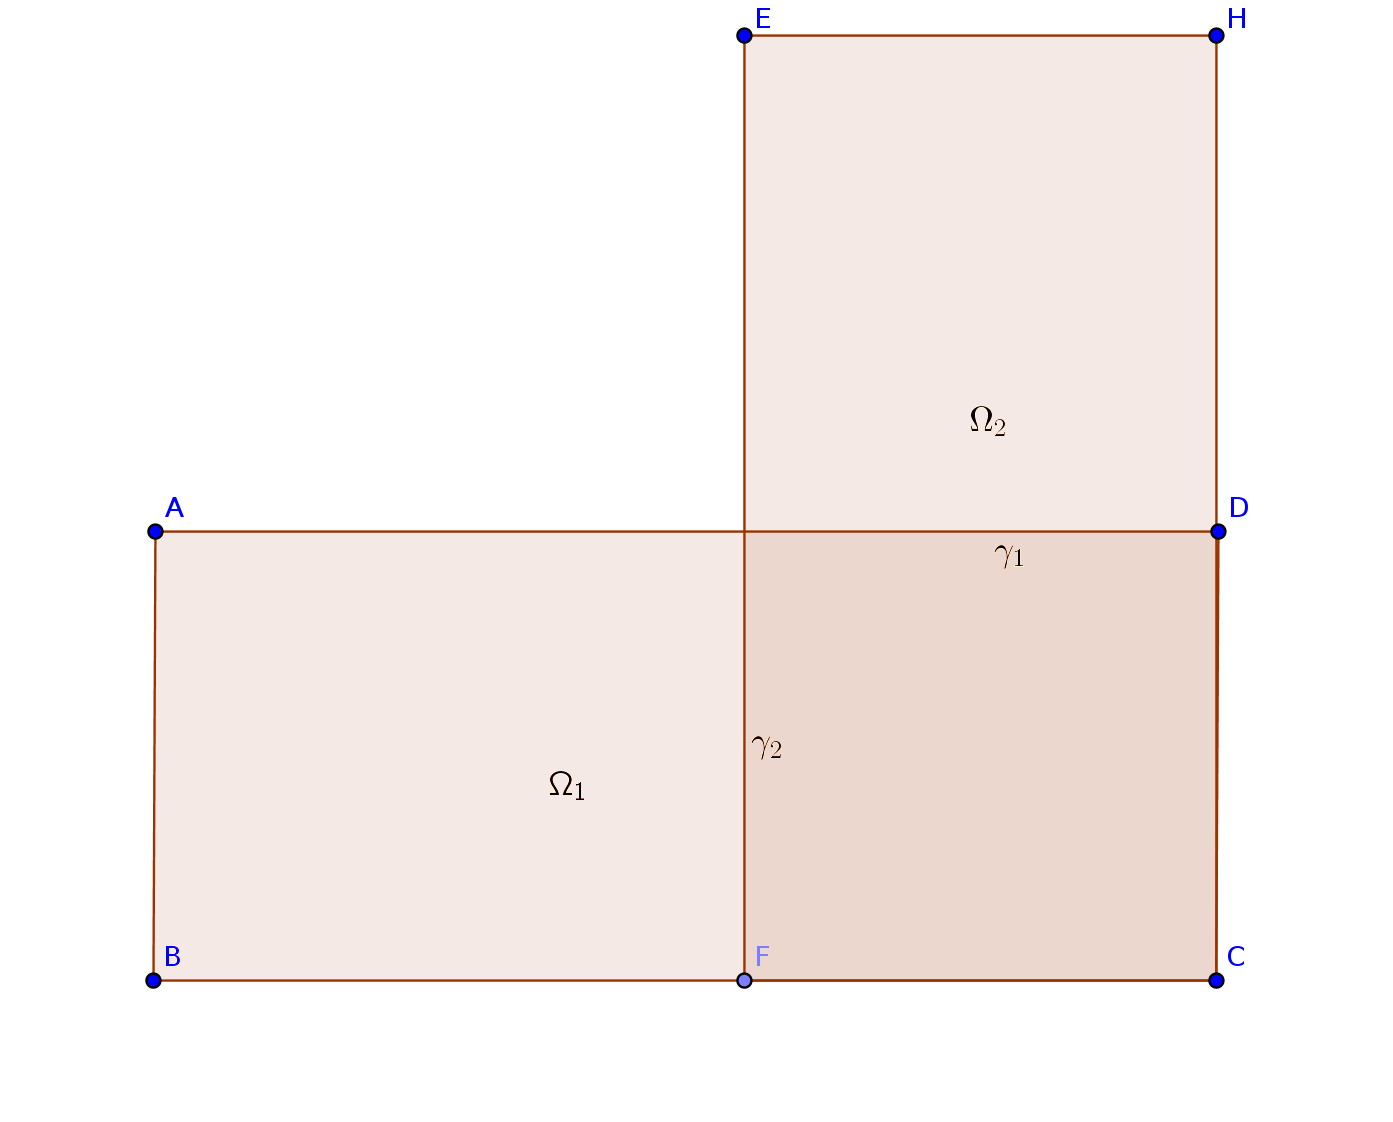
\includegraphics[width=140mm,scale=0.4]
{lshapedomain.png}
\end{figure}
We first show that $Y=Y_1+Y_2$ is a proper subspace of $X$. Assume for contradiction that $X=Y_1+Y_2$, then for each $u\in X$, we have $u=u_1+u_2$ where $u_1\in Y_1$, $u_2\in Y_2$. Now we consider the trace defined as
$$\mathrm{Tr}\colon H^{1} \to H^{\frac{1}{2}}(\partial \Omega).$$
Since $u\equiv 1\in H^1(\Omega)$ and $u$ is continuous on $\overline{\Omega}$, then 
$$1=\mathrm{Tr}u=\mathrm{Tr}(u_1+u_2)=\mathrm{Tr}u_1+\mathrm{Tr}u_2.$$

We also have $\mathrm{Tr}u_1=0$ on $\partial\Omega_1$, and $\mathrm{Tr}u_2=0$ on $\partial\Omega_2$, so $\mathrm{Tr}u_2=1$ on $\gamma_1$ and $\mathrm{Tr}u_1=1$ on $\gamma_2$. This implies that $\mathrm{Tr}u_1=\mathbbm{1}_{\gamma_2}$ on $\gamma_1\cup\gamma_2$, but $\mathbbm{1}_{\gamma_2}\notin H^{\frac{1}{2}}(\gamma_1\cup\gamma_2)$ as
$$\int_{(\gamma_1\cup\gamma_2)}\int_{(\gamma_1\cup\gamma_2)}\frac{|\mathbbm{1}_{\gamma_2}(x)-\mathbbm{1}_{\gamma_2}(y)|^2}{|x-y|} dx dy=\infty,$$
thus yields a contradiction.

\par
Now we proceed to the density argument. Note that for each $u\in Y=Y_1+Y_2$, for $\varepsilon>0$,  there exists $\varphi_i\in Z_i$ such that $$\|u-\varphi_1-\varphi_2\|_{H^1}<\varepsilon.$$ Define
$Z:=\{\varphi \in C^{\infty}(\Omega)\colon \varphi=0 \mbox{ near the problematic point}\}$, then $Z=Z_1+Z_2$.
 It suffices to show that for each $u\in C^{\infty}(\Omega)$, for all $\varepsilon>0$, there exists $\varphi\in Z$ such that $\|u-\varphi\|_{H^1}<\varepsilon$. Assume that $z$ is the probematic point, and consider the function $\varphi_{\varepsilon}\colon \Omega\to\mathbb{C}$ defined as 
$$\varphi_{\varepsilon}(x,y)=\begin{cases} \left(\frac{|(x,y)-z|}{\varepsilon}\right)^{\varepsilon}, \mbox{ for } r=|(x,y)-z|\in(0,\varepsilon), \\
1,  \mbox{ otherwise}.\\
\end{cases}$$
For each $u\in C^{\infty}(\Omega)$, we have $u_{\varepsilon}:=u\cdot \varphi_{\varepsilon}\in \tilde{Z}:=\{\varphi\in C^1(\Omega),\varphi=0 \mbox{ near the problematic point}\}$. Since $Z$ is dense in $\tilde{Z}$, it suffices to show that $\|u-u_{\varepsilon}\|_{H^1}\to 0$ as $\varepsilon\to\infty$. Note that
$$\|u-u_{\varepsilon}\|_{L^2}\rightarrow 0 \mbox{ as } \varepsilon\rightarrow 0,$$ and 
\begin{align*}
\|\bigtriangledown u-\bigtriangledown u_{\varepsilon}\|_{L^2}&=\| \bigtriangledown u (1-\varphi_{\varepsilon})-u\bigtriangledown \varphi_{\varepsilon}\|_{L^2}\\
{}&\leq C(\|1-\varphi_{\varepsilon}\|_{L^2}+\|\bigtriangledown \varphi_{\varepsilon}\|_{L^2})
\end{align*}
for some positive constant $C$. It is obvious that $\|1-\varphi_{\varepsilon}\|_{L^2}\to 0$ as $\varepsilon\to 0$.
Also,
\begin{align*}
\|\bigtriangledown\varphi_{\varepsilon}(x,y)\|_{L^2}&=\| \bigtriangledown \varphi_{\varepsilon}(r)\|_{L^2}\\
{}&= \| \left(\frac{r}{\varepsilon}\right)^{\varepsilon-1}(\cos\theta, \sin\theta)\|_{L^2}\\
{}&=\left(\int_{0}^{\varepsilon}\int_{0}^{2\pi} \left(\frac{r}{\varepsilon}\right)^{2\varepsilon-2} r dr d\theta\right)^{\frac{1}{2}}\\
{}&=\sqrt{2\pi}\left(\int_{0}^{\varepsilon}\left(\frac{r}{\varepsilon}\right)^{2\varepsilon-2} r dr\right)^{\frac{1}{2}}\\
{}&=\sqrt{2\pi} \sqrt{\frac{\varepsilon}{2}}\\
{}&=\sqrt{\pi \varepsilon}
\end{align*}
tends to $0$ as $\varepsilon\to 0$.
Thus, $\|u-u_{\varepsilon}\|_{H^1}=\|u-u_{\varepsilon}\|_{L^2}+\|\bigtriangledown  u-\bigtriangledown u_{\varepsilon}\|_{L^2}\to 0$ as $\varepsilon\to 0$.
\end{proof}
\end{lemma}


\section{Demonstration of the rate of convergence in Matlab}\label{sec:matlab}
In this section, we analyse the rate of convergence by comparing the plots of error norms against the number of iterations.

In section \ref{sec:dichotomy results}, we have proved the \emph{Von-Neumann Halperin Dichotomy} which states that:

If $M_i$  ($1\leq i\leq r$ ) are closed subspaces in the Hilbert space $X$, and $M:=\bigcap_{i}^r M_i$, then for $T=P_{r}P_{r-1}\cdots P_{1}$ where $P_{i}$ is the orthogonal projection on $M_i$, exactly one of the two following statements holds:
\begin{enumerate}
\item $\sum_{i=1}^r M_{i}^{\perp}$ is closed, then there exists $\alpha\in [0,1)$ and $c\in \mathbb{R}$ such that $\|T^n-P_{M}\|\leq c\alpha^n$ for each $n$.
\item $\sum_{i=1}^r M_{i}^{\perp}$ is not closed, then for each $(r_n)\in c_0$, $r_n\in\mathbb{R}^{+}$, for all $x\in X$, $\|T^n x-P_{M}x\|\neq O(r_n)$.
\end{enumerate}

In fact, we can replace (b) by arbitrarily slow convergence, that is,
for each $(r_n)\in c_0$, $r_n\in\mathbb{R}^{+}$, there exists $x\in X$ such that $\|T^n x-P_{M}x\|\geq r_n$ for each $n\in\mathbb{N}$\cite{DH10a}. 

In \emph{Deusch} and \emph{Hundal's} recent work\cite{DH15}, they suggest  that the $x\in X$ satisfies $\|T^n x-P_{M}x\|\geq r_n$ for all $n$ must be chosen from $X\setminus(M\oplus(M_1^{\perp}+M_2^{\perp}))$.

In the application of Schwarz Altenrating Method for the Neumann problem in the two-dimensional domain, we have showed that $M=\{0\}$, so the $x$ have to be chosen from $H^1(\Omega)\setminus (M_1^{\perp}+M_2^{\perp})$.

In order to test the above conjecture, we claim that for $u\in C(\overline{\Omega})\cap(M_1^{\perp}+M_2^{\perp})$, we have $u(x)=0$ for all problematic points on $\partial\Omega$.  The claim is indeed true due to the following fact: if $u\in C(\overline{\Omega})\cap H^1(\Omega)$, then there exists $\phi_n\in C^{\infty}(\overline{\Omega})$ such that $\|u-\phi_n\|_\infty\rightarrow 0$ as $n\rightarrow \infty$.

Since $u\in C(\overline{\Omega})\cap(M_1^{\perp}+M_2^{\perp})=C(\overline{\Omega})\cap (Y_1+Y_2)=C(\overline{\Omega})\cap Y=C(\overline{\Omega})\cap \overline{Z}$ where $$Z=\{u\in C^{\infty}, u=0 \mbox{ near the problematic points}\},$$ there exists $u_n\in C^{\infty}(\overline{\Omega})\cap Z$ such that $\|u-u_n\|_{\infty}\rightarrow 0$ as $n\rightarrow \infty$.  $u_n=0$ on problematic points implies that $u(x)=\lim_{n\rightarrow} u_n(x)=0$ for all problematic points on $\partial \Omega$. 

Thus for $x_0\in H^1(\Omega)\setminus (M_1^{\perp}+M_2^{\perp})$, we need $x_0\neq 0$ at problematic points, that is, $u_0\neq u$ at problematic points for $u, u_0\in H^1(\Omega)$.


Consider the neumann problem 
$$\begin{cases}
-\Delta u+u=1, \\
\frac{\partial u}{\partial r}=0\\
\end{cases}$$
on a L-shape domain as shown in Figure 4.1.
\begin{figure}[t]
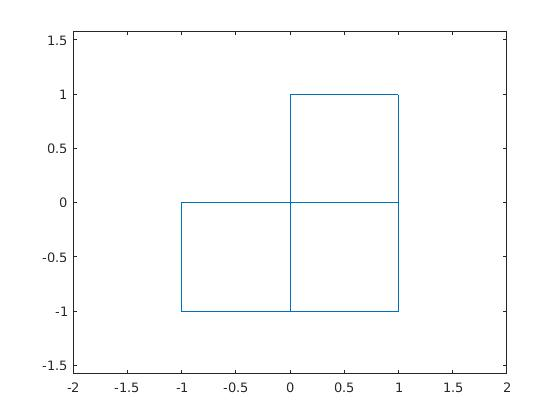
\includegraphics[width=\textwidth]{lshape.jpg} 
\caption{lshape domain}
\end{figure}

It is easy to see that the true solution is $u\equiv 1$. 

If we set $u_0=|\log(\frac{1}{\sqrt{(x^2+y^2)}})|^\alpha$ for $\alpha\in (0,0.5)$, $u_0=\infty$ at the problematic point $(0,0)$, then the surface plot of the solution after $80$ iterations is shown in Figure 4.2. (Details of the Matlab code can be found in Appendix \ref{sec:appA})

\begin{figure}[h]
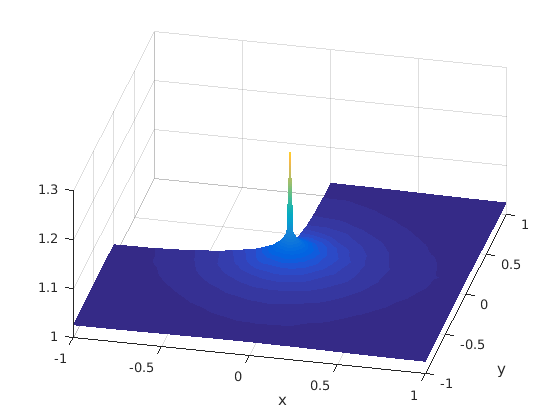
\includegraphics[width=\textwidth]{verybadinitial_u.png}
\caption{surface plot of the solution $u_n$}
\end{figure}

We plot both $\log(\|u_n-u\|_\infty)$ and $\log(\|u_n-u\|_{H1})$ against the number of iterations with respect to different mesh sizes to demontrate the rate of convergence.

\begin{figure}[h]
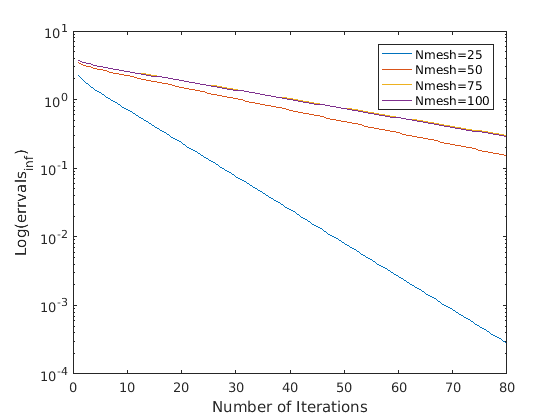
\includegraphics[width=\textwidth]{verybadinitial_infnorm.png}
\caption{The plots of $\log(\|u_n-u\|_\infty)$ against number of iterations}
\end{figure}
\begin{figure}[h]
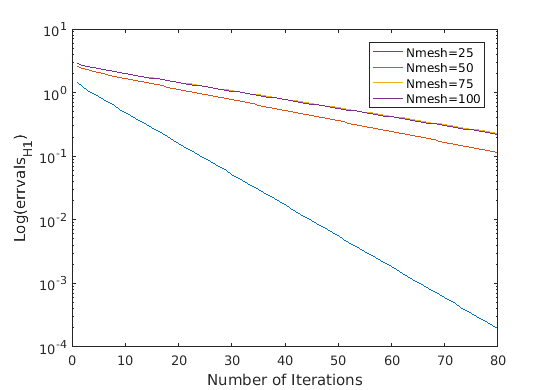
\includegraphics[width=\textwidth]{verybadintial_H1norm.png}
\caption{The plots of $\log(\|u_n-u\|_{H1})$ against number of iterations }
\end{figure}

As we can observe from Figure 4.3 and Figure 4.4, the rate of convergence decays as the number of iterations increase with respect to both the infinity and $H_1$ norms. The results shown on the two error plots are compatible with \emph{Deutsch} and \emph{Hundal's} conjecture.

From the plots we can also deduce that the rate of convergence decreses when we refine the mesh near the problematic point. After we refine the mesh to a certain scale (i.e.Nmesh$=75$ in our plot), the plot will no longer depend on the mesh size.

\begin{figure}[h]
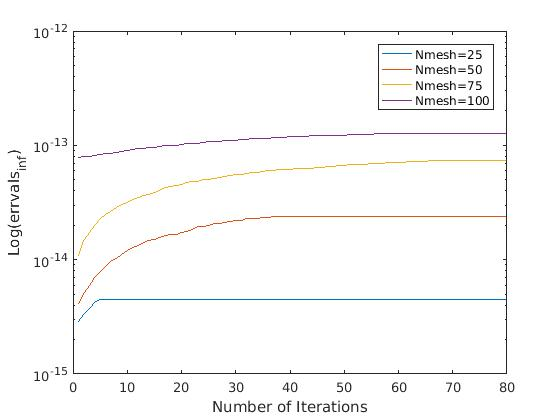
\includegraphics[width=\textwidth]{goodinitial_inf.jpg}
\caption{The plots of $\log(\|u_n-u\|_{\infty})$ against number of iterations }
\end{figure}

Now we start with a good initial guess, $u_0=1-\sin(22x)sin(10y)$, which gives $u_0=1$ on the problematic point. Again, we plot the two error norms against the number of iterations.
\begin{figure}[h]
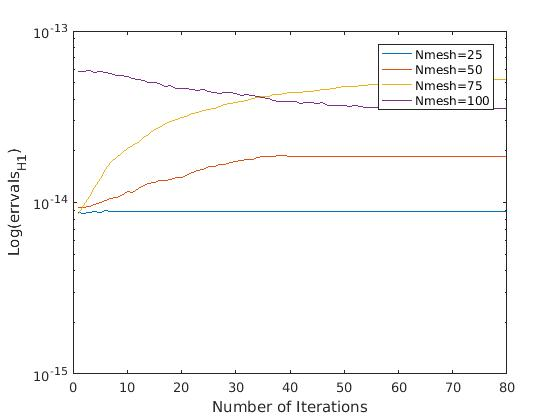
\includegraphics[width=\textwidth]{goodinitial_H1.jpg}
\caption{The plots of $\log(\|u_n-u\|_{H1})$ against number of iterations }
\end{figure}
 
From \emph{Deutsch} and \emph{Hundal's} conjecture, we expect exponentially fast convergence, that is, straight lines for the plots of both $\log(\|u-u_n\|_{\infty})$ and $\log(\|u-u_n\|_{H1})$ against the number of iterations.
However, the plots shown on Figure 4.5 and Figure 4.6 are bizarre for the first few iterations. I suspect that this is because the numerical solutions we obtained from solving PDEs on different domains are approximate values only. Since the soluitons are pointwise values, we try to decrease our grid size, that is, to increase the number of plots ( change Nplot$=101$ to Nplot=$2001$) to increase their accuracy.  We plot the first few iterations in Figure 4.7 and Figure 4.8 to see whether there is any improvement. 
\begin{figure}[h]
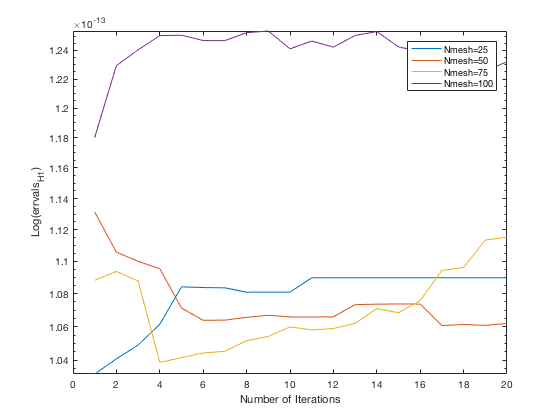
\includegraphics[width=\textwidth]{smallgridsize.png}
\caption{The plots of $\log(\|u_n-u\|_{H1})$ against number of iterations }
\end{figure}
\begin{figure}[h]
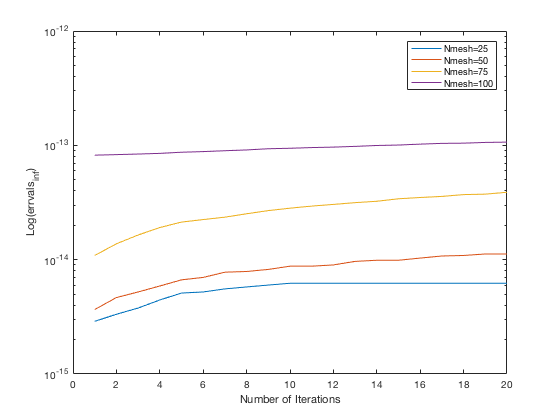
\includegraphics[width=\textwidth]{smallgridsize2.png}
\caption{The plots of $\log(\|u_n-u\|_{\infty})$ against number of iterations }
\end{figure}
\par
Surprisingly, the plots are inconsistent with what we expect as well. In fact, the plots are reasonable in some sense since the errors are quickly within machine precision. 

\chapter{Conclusion}\label{chapt:conclusion}
In this paper, our main focus was the \emph{Schwarz Alternating Method} for the two-dimensional Poisson's equation with Neumann boundary conditions. In fact, this iterative approach also applies to other different classes of equations such as Stokes equations and nonlinear variants, and more details can be found in \emph{Lion's} 1988 paper \cite{PL88}. Moreover, we can also extend from two subdomains to any fintie number of subdomains. The convergence result follows from the  \emph{von-Neumann Halperin Theorem}, while the algorithm is very similiar to our two dimensional case.

In the numerical analysis section of this paper, we restricted the application of our algorithm to a specific L-shaped domain for simplicity, but I believe that our  Matlab code can also be adapted for any composite domain which is a union of two subdomains with uniform overlapping.


%Furthermore, von Neumann's alternating projections algorithm can also be applied in many other areas, such as interpolation of stochastic processes \cite{•},\cite{•},\cite{•}, reconstruction of images in medicine and geogphysics\cite{•},\cite{•}, and some other applications mentioned by \emph{Deutsch} \cite{De83}.


\chapter{Appendices}\label{chapt:appendices}
\section{Appendix A}\label{sec:appA}
\begin{verbatim}
tic;
Nsteps = 80;   % Number of iterations
Nplot = 101;   % Fineness of plots
T = 10*eps;   % Time delay
az = 13;      % Plot viewing angle
el = 48;      % Plot viewing height
v = 0.0;      % Camera speed
fix_axes = 0;               % Set to 1 for fixed axes
plot_range = [-0.1 1.1];    % z-axis range if fixed
% col_range = plot_range;   % Fixed colour range
% col_range = [-.7 1.1];
col_range = 'manual';       % Varying colour range
rec = 0;                    % record on/off
xg = linspace(-1,1,Nplot);
yg = linspace(-1,1,Nplot);
[XX,YY] = meshgrid(xg,yg);
ZZ = NaN(size(XX));

[indy_up,indx_up]=find(XX>=0);
indx_up = unique(indx_up);
indy_up = unique(indy_up);

[indy_lo,indx_lo]=find(YY<=0);
indx_lo = unique(indx_lo);
indy_lo = unique(indy_lo);

indices_all=find(XX>=0|YY<=0);
ZZ(indices_all)=1;
Du_dy=(ZZ(1:Nplot-2,:)-ZZ(3:Nplot,:));
Du_dx=(ZZ(:,3:Nplot)-ZZ(:,1:Nplot-2));
diffy_ind=~isnan(Du_dy);
diffx_ind=~isnan(Du_dx);
\end{verbatim}


\subsection*{Export geometry}

\begin{verbatim}
load('upper_rectangle')
load('lower_rectangle')
\end{verbatim}


\subsection*{Define the problem}

\begin{verbatim}
a = 1;
c = 1;        % Coeffs in PDE
f = 1;        % RHS of PDE
% f = '1+x.^2+12*(y+1)';
% f = '1./(x.^2+(y+1/2).^2)-1./((x-1/2).^2+y.^2)';

initguess=@(x,y) abs(log(1./((x.^2+y.^2).^.5))).^0.4999 % u0=infinity
% initguess=@(x,y) 1;
% initguess = @(x,y) 0; % u0~=1 @(0,0)
% initguess = @(x,y) -1-sin(22*x).*sin(10*y);
% initguess = @(x,y) 1-sin(22*x).*sin(10*y);
% initguess = @(x,y) 0.0+(min(x.^2+(y+.5).^2,(x-.5).^2+y.^2)<.005);
% initguess = @(x,y) (min(x.^2+(y+.5).^2,(x-.5).^2+y.^2)>.05);
% initguess = @(x,y) -3+4*(x.^2+(y+1/2).^2>.001);
% initguess = @(x,y) 1-.001./(x.^2+(y+1/2).^2).^(1/3)-.001./((x-1/2).^2+y.^2).^(1/3);
%initguess = @(x,y) 10-7.*(abs(log(-x.^2-(y+1/2).^2))).^0.4999;
\end{verbatim}
\subsection*{Generate the mesh}

\begin{verbatim}
errvals_inf= zeros(4,Nsteps);
errvals_H1=zeros(4,Nsteps);

for Nmesh=25:25:100;
\end{verbatim}
\begin{verbatim}
meshgenfun = '1./(x.^2+y.^2)'; % function for adaptive mesh generation
[~,p_up,e_up,t_up]=adaptmesh(g_up,b_up,c,a,meshgenfun,'Ngen', Nmesh);
[~,p_lo,e_lo,t_lo]=adaptmesh(g_lo,b_lo,c,a,meshgenfun,'Ngen', Nmesh);
figure(1);
pdemesh(p_up,e_up,t_up);
xlim ([-1.5,1.5]);
axis equal;

figure(2);
pdemesh(p_lo,e_lo,t_lo);
xlim ([-1.5,1.5]);
axis equal;
\end{verbatim}

   
      
    
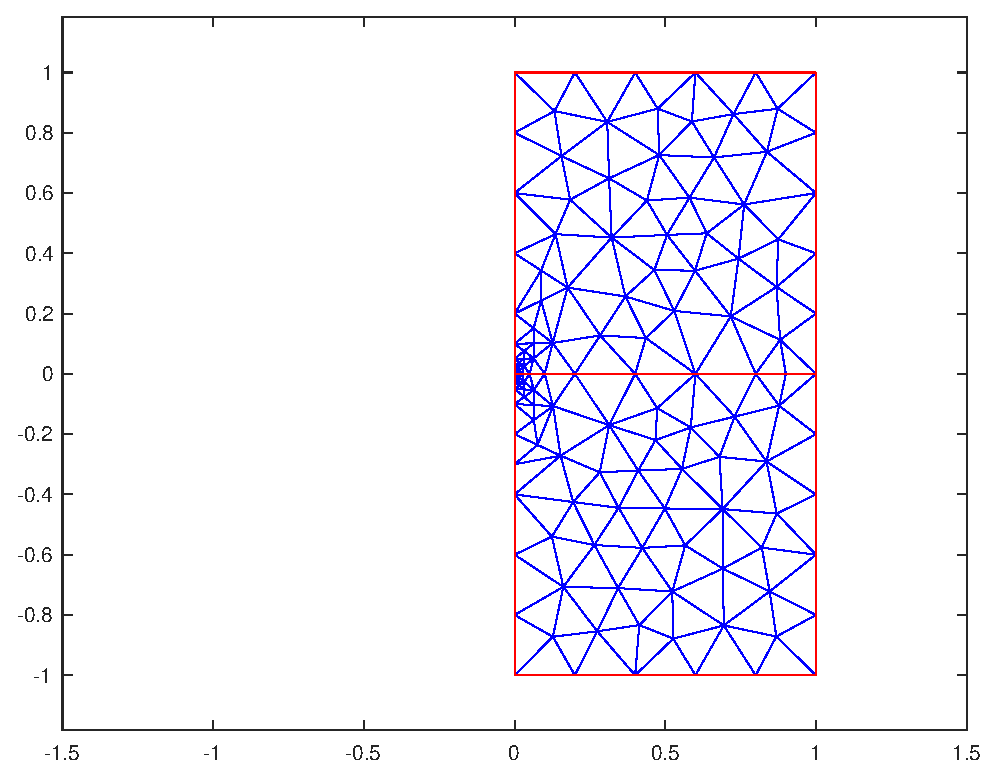
\includegraphics [width=4in]{lshape_neumann_meshsize2_01.eps}

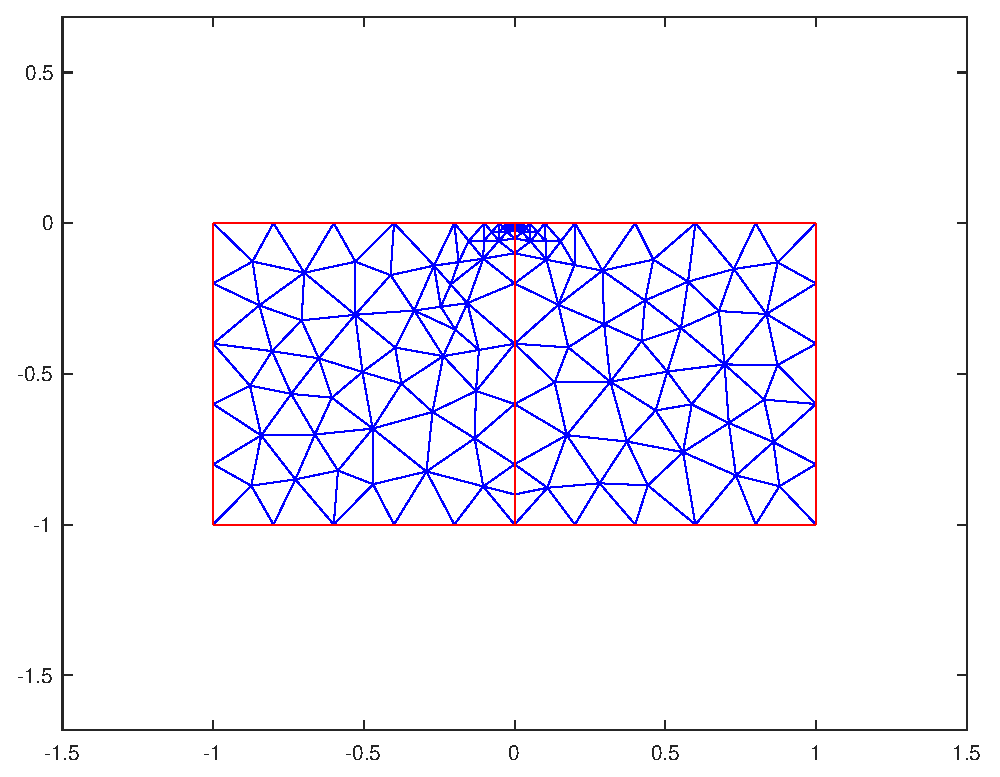
\includegraphics [width=4in]{lshape_neumann_meshsize2_02.eps}

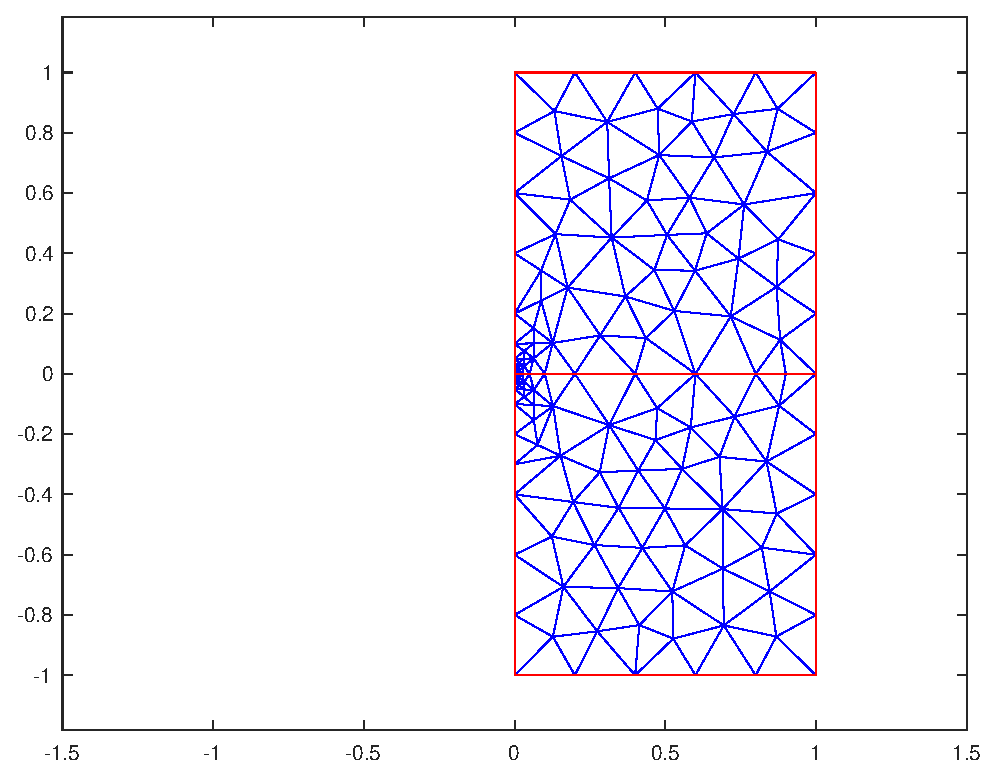
\includegraphics [width=4in]{lshape_neumann_meshsize2_04.eps}

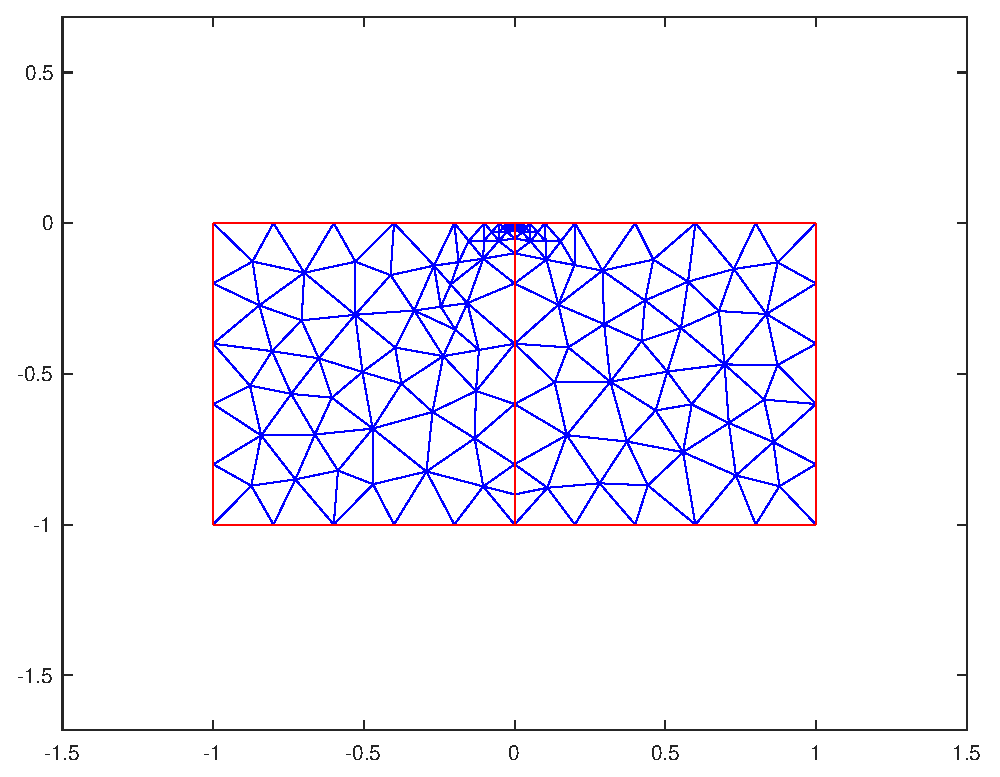
\includegraphics [width=4in]{lshape_neumann_meshsize2_05.eps}

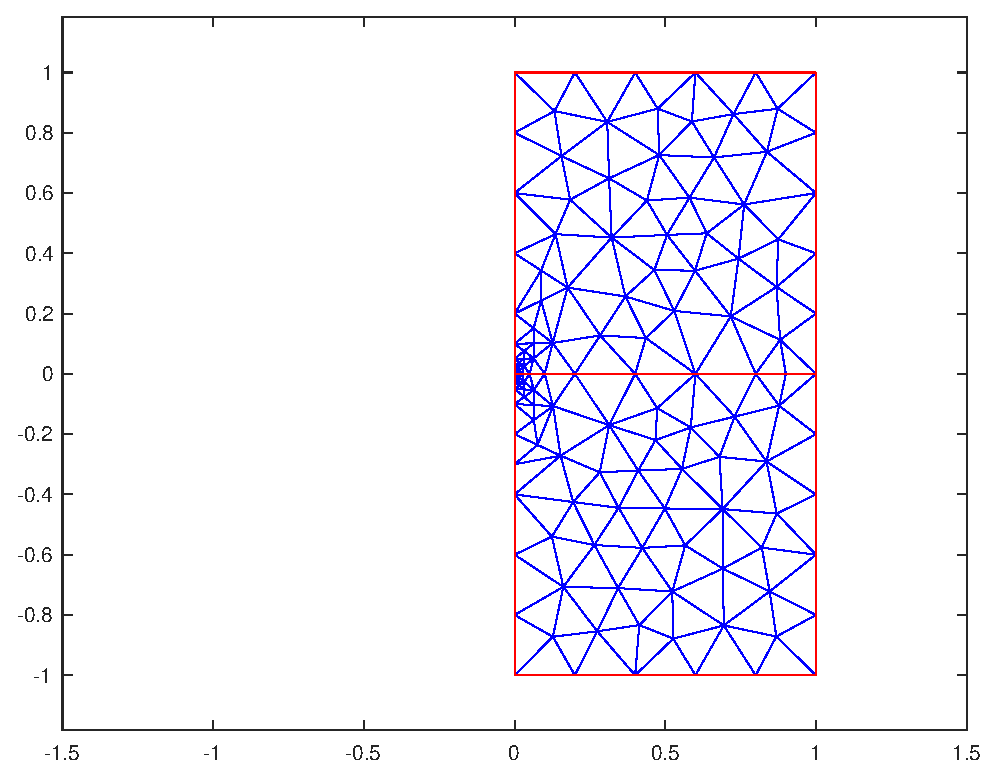
\includegraphics [width=4in]{lshape_neumann_meshsize2_07.eps}

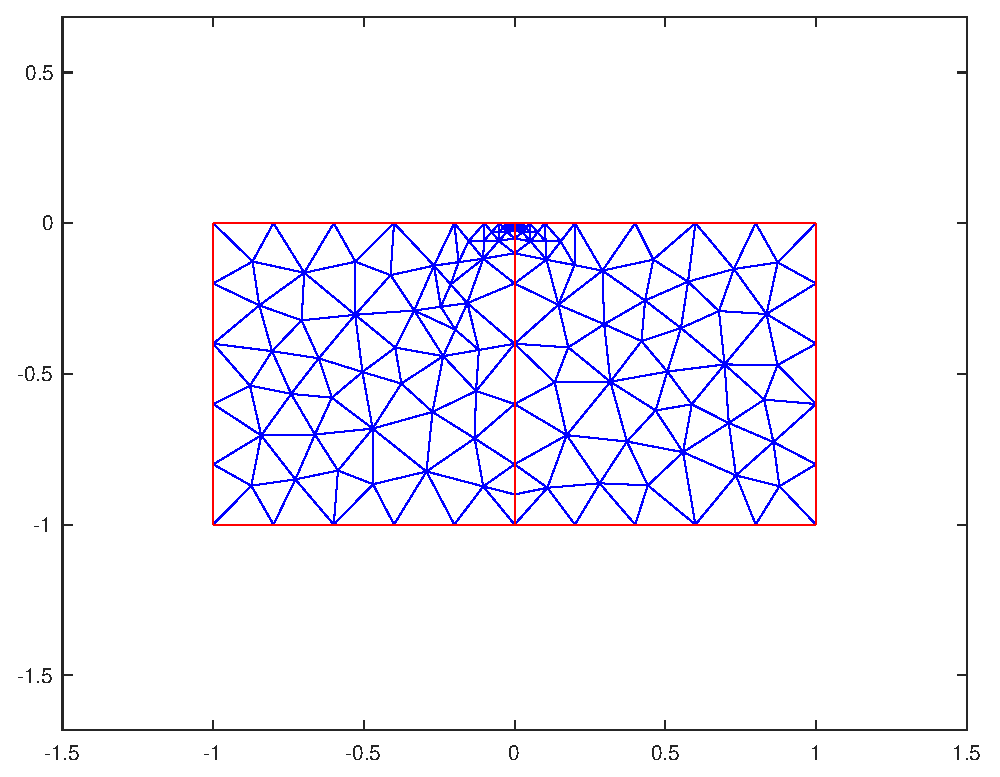
\includegraphics [width=4in]{lshape_neumann_meshsize2_08.eps}

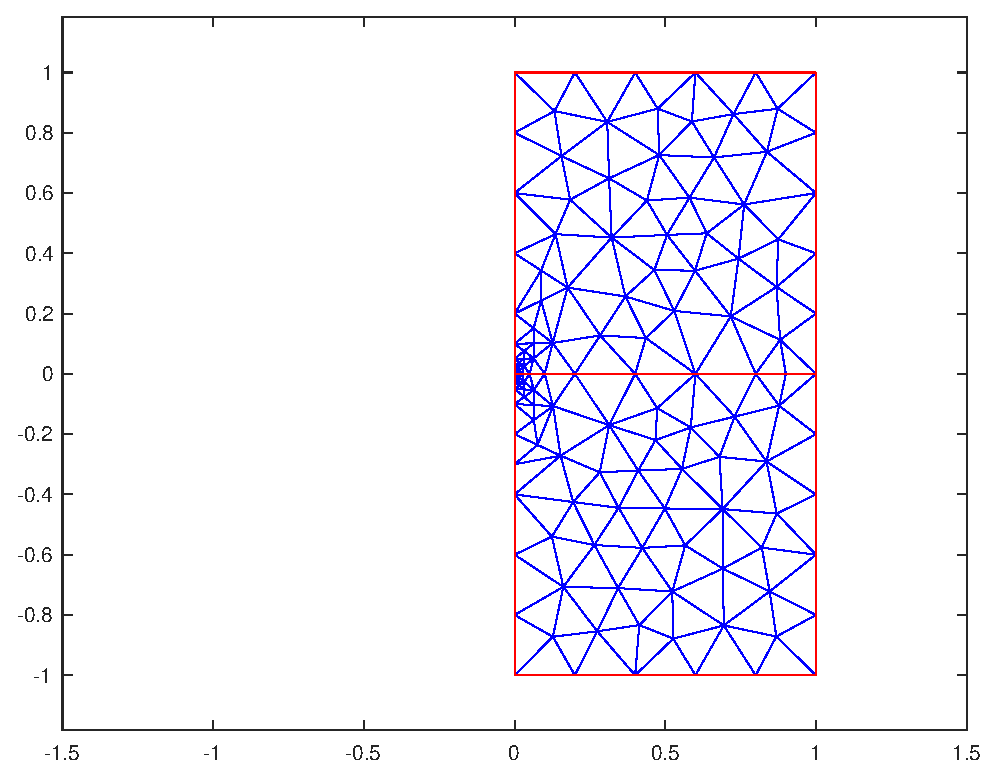
\includegraphics [width=4in]{lshape_neumann_meshsize2_10.eps}

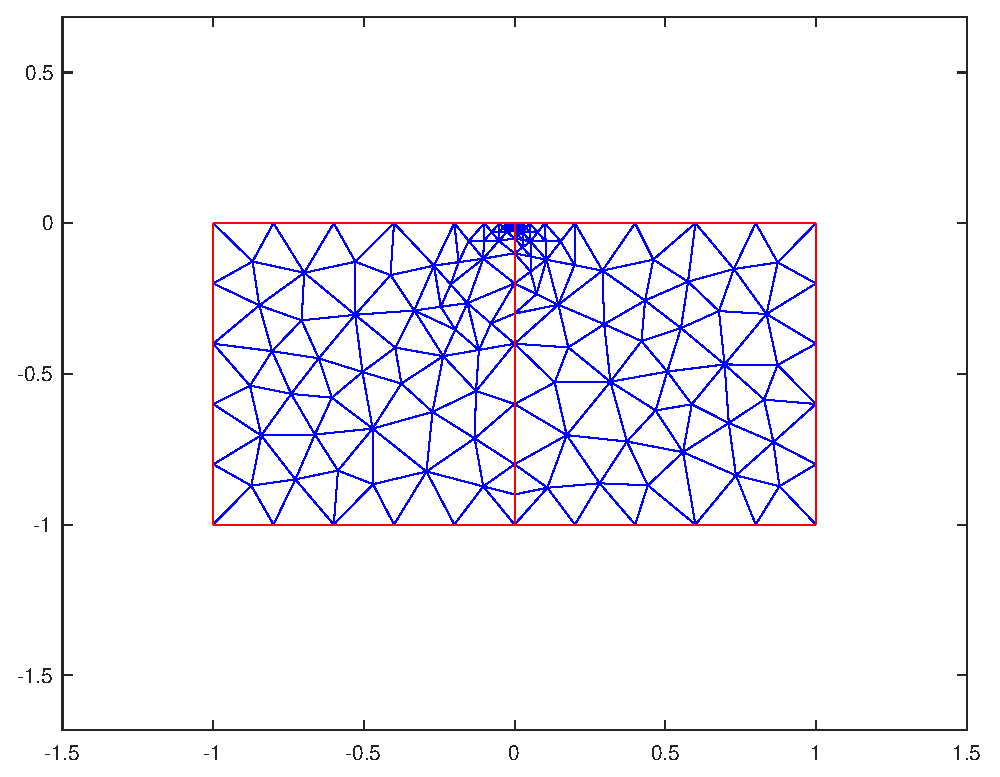
\includegraphics [width=4in]{lshape_neumann_meshsize2_11.eps}


\subsection*{Obtain relative matrices}

\begin{verbatim}
[K_up,M_up,F_up,Q_up,G_up,H_up,R_up]=assempde(b_up,p_up,e_up,t_up,c,a,f);
[K_lo,M_lo,F_lo,Q_lo,G_lo,H_lo,R_lo]=assempde(b_lo,p_lo,e_lo,t_lo,c,a,f);
\end{verbatim}


\subsection*{Assign true solution}

\begin{verbatim}
u_up_true = ones(1,length(p_up));
u_lo_true = ones(1,length(p_lo));
\end{verbatim}


\subsection*{Iterations}

\begin{verbatim}
counter = 0;
if rec == 1
    Vid = VideoWriter('Temp_video', 'MPEG-4');
    Vid.FrameRate = 3;
    Vid.Quality = 100;
    open(Vid);
end
ZZ(XX>=0) = initguess(XX(XX>=0),YY(XX>=0));
ZZ(YY<=0) = initguess(XX(YY<=0),YY(YY<=0));
figure(3);
my_plot_new(XX,YY,ZZ,az,el,v, plot_range, col_range,0,fix_axes);

if rec == 1
    frame = getframe(gcf);
    writeVideo(Vid,frame);
end
pause

% Note that pind_up2 represents the indices of the mesh points at the boundary in the
% upper domain
[pind_up1,pind_up2]=find(H_up);
% Remove the problematic point
ind=find((abs(p_up(1,pind_up2) -0)<1e-10) & (abs(p_up(2,pind_up2) -0)<1e-10));
pind_up1(ind)=[];
pind_up2(ind)=[];
% Update the Dirichlet condition matrix H_up
H_up=H_up(pind_up1,:);


[pind_lo1,pind_lo2]=find(H_lo);
% Remove the problematic point
ind=find((abs(p_lo(1,pind_lo2) -0)<1e-10) & (abs(p_lo(2,pind_lo2) -0)<1e-10));
pind_lo1(ind)=[];
pind_lo2(ind)=[];
% Update the Dirichlet condition matrix H_lo
H_lo=H_lo(pind_lo1,:);


bnew_up=zeros(length(pind_up2),1);
bnew_lo=zeros(length(pind_lo2),1);

for step = 1:Nsteps;
    if step == 1
        bfun_up = @(x,y) initguess(x,y);
    else
        bfun_up = @(x,y) tri2grid(p_lo,t_lo,u_lo,x,y);
    end
% Update  boundary conditions
for i=1:length(pind_up2);
    bnew_up(i)=bfun_up(p_up(1,pind_up2(i)),p_up(2,pind_up2(i)));
end
% Update the Dirichlet condtion vector R_up
 R_up = H_up(:,pind_up2)*bnew_up;

% Solve the pde in the upper domain
u_up=assempde(K_up,M_up,F_up,Q_up,G_up,H_up,R_up);

% Plot the solution
ZZ(XX>=0) = tri2grid(p_up,t_up,u_up,xg(indx_up),yg(indy_up));
figure(3);
my_plot_new(XX,YY,ZZ,az,el,v, plot_range, col_range, counter,fix_axes);

if rec == 1
    frame = getframe(gcf);
    writeVideo(Vid,frame);
end

pause(T)
counter = counter+1;

bfun_lo = @(x,y) tri2grid(p_up,t_up,u_up,x,y);

% Update the boundary conditions
for i=1:length(pind_lo2);
    bnew_lo(i)=bfun_lo(p_lo(1,pind_lo2(i)),p_lo(2,pind_lo2(i)));
end

% Update the Dirichlet condition vector
R_lo = H_lo(:,pind_lo2)*bnew_lo;

% Solve the pde in the lower domain
u_lo=assempde(K_lo,M_lo,F_lo,Q_lo,G_lo,H_lo,R_lo);

%Plot the solution
ZZ(YY<=0) = tri2grid(p_lo,t_lo,u_lo,xg(indx_lo),yg(indy_lo));
figure(3)
my_plot_new(XX,YY,ZZ,az,el, v, plot_range, col_range, counter,fix_axes);

if rec == 1
    frame = getframe(gcf);
    writeVideo(Vid,frame);
end

pause(T)

counter = counter+1;

% The error calculated with respect to infinity norm
errvals_inf(Nmesh/25,step)=max(max(abs([u_up(:); u_lo(:)]-[u_up_true(:); u_lo_true(:)])));

% The error calculated with respect to H1 norm

% The difference between the solution from ASM and the true solution
u_diff=ZZ-ones(size(ZZ));
% Square the difference
u_diff_square=u_diff.*u_diff;
%  stepsize on x-axis
dx=(1-(-1))/(Nplot-1);
% stepsize on y-axis
dy=(1-(-1))/(Nplot-1);
integral_1=sum(sum (dx*dy*u_diff_square(indices_all)));

% Approximate the derivatives by Central Difference Method
Du_dy=(ZZ(3:Nplot,:)-ZZ(1:Nplot-2,:))/(2*dy);
Du_dx=(ZZ(:,3:Nplot)-ZZ(:,1:Nplot-2))/(2*dx);
% Integrate on the y-direction
integrand_y=Du_dy.*Du_dy*dx*dy;
% Integrate on the x-direction
integrand_x=Du_dx.*Du_dx*dx*dy;
integrals=[integral_1,sum(sum(integrand_y(diffy_ind))),sum(sum(integrand_x(diffx_ind)))];
errvals_H1(Nmesh/25,step)=sqrt(sum(integrals));
end
\end{verbatim}

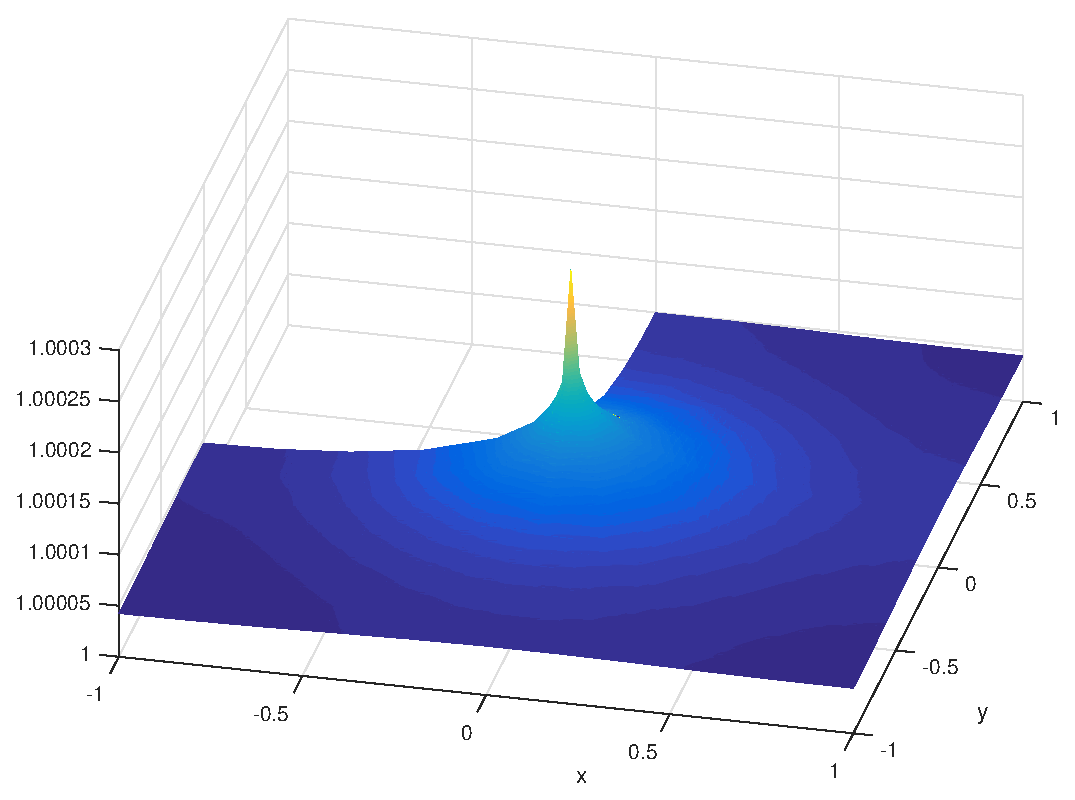
\includegraphics [width=4in]{lshape_neumann_meshsize2_03.eps}

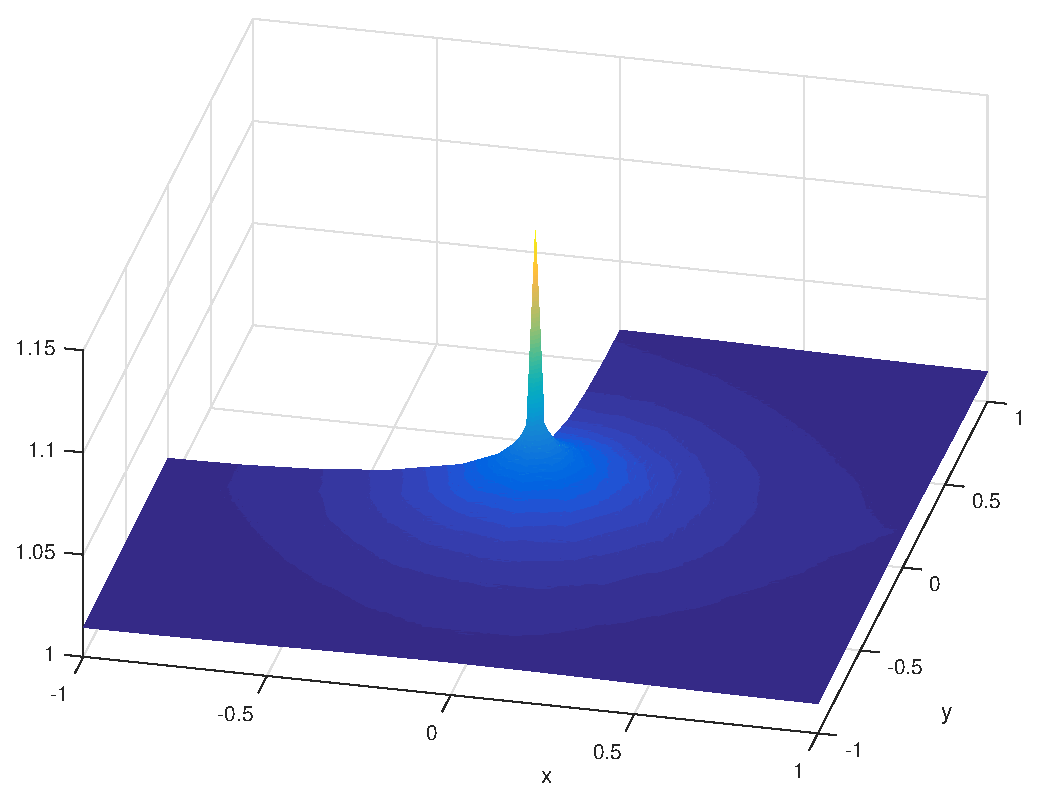
\includegraphics [width=4in]{lshape_neumann_meshsize2_06.eps}

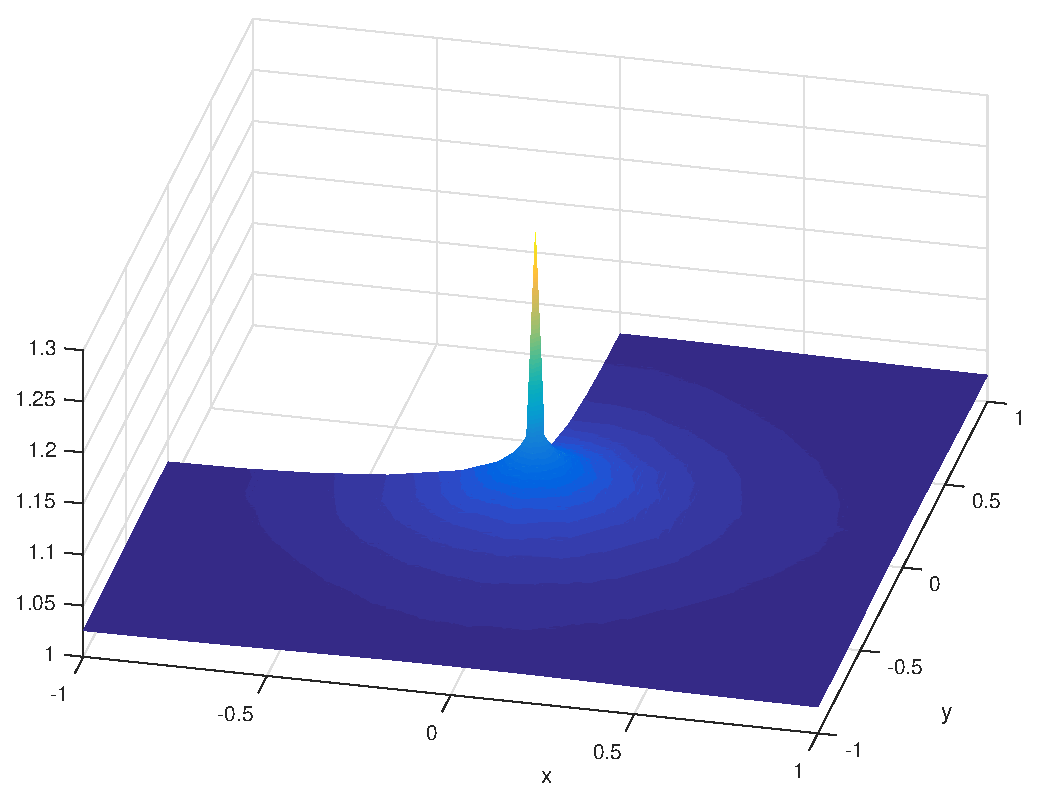
\includegraphics [width=4in]{lshape_neumann_meshsize2_09.eps}

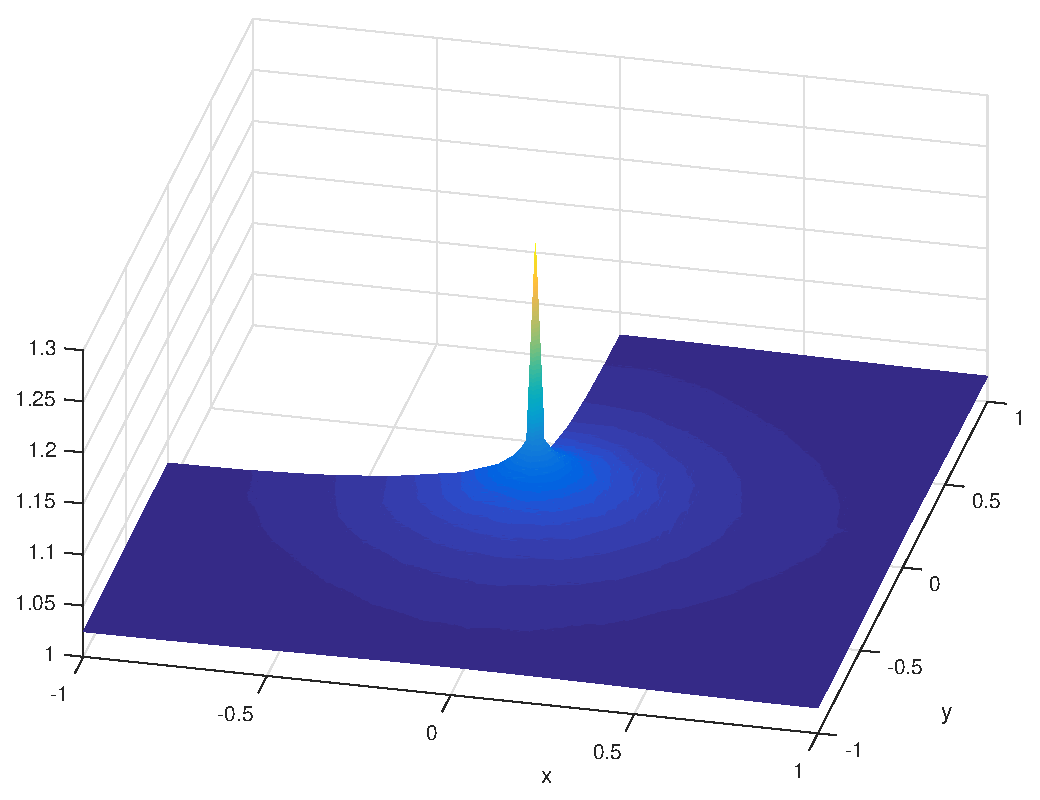
\includegraphics [width=4in]{lshape_neumann_meshsize2_12.eps}
\begin{verbatim}
end

if rec == 1
    close(Vid);
end
\end{verbatim}


\subsection*{Plot of \texttt{\ensuremath{|}u\_n-u\_true}\ensuremath{|} versus Nsteps}

\begin{verbatim}
figure(4)
nn = 1:Nsteps;
semilogy(nn,[errvals_inf(1,:);errvals_inf(2,:);errvals_inf(3,:);errvals_inf(4,:)]);
legend('Nmesh=25','Nmesh=50', 'Nmesh=75','Nmesh=100')
xlabel('Number of Iterations'); % x-axis label
ylabel('Log(errvals_{inf})') ;    % y-axis label

figure(5)
nn = 1:Nsteps;
semilogy(nn,[errvals_H1(1,:);errvals_H1(2,:);errvals_H1(3,:);errvals_H1(4,:)]);
legend('Nmesh=25','Nmesh=50', 'Nmesh=75','Nmesh=100');
xlabel('Number of Iterations'); % x-axis label
ylabel('Log(errvals_{H1})');     % y-axis label
toc
\end{verbatim}

        \color{lightgray} \begin{verbatim}Elapsed time is 90.622654 seconds.
\end{verbatim} \color{black}
    
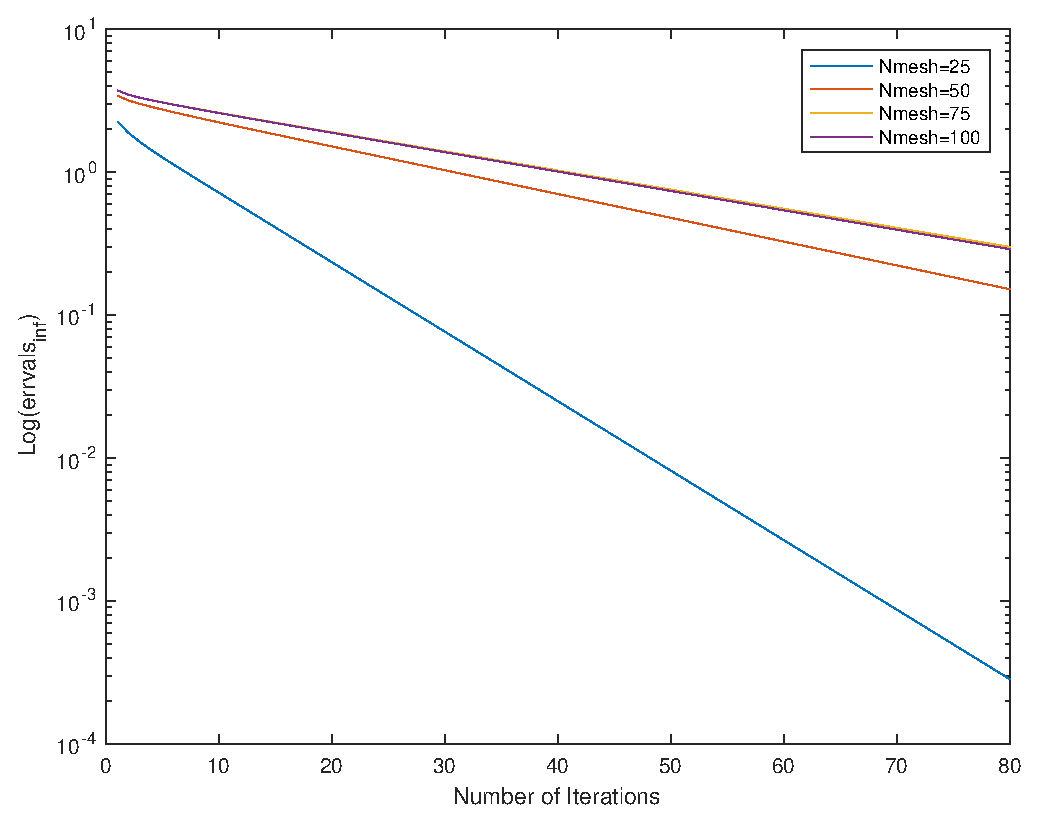
\includegraphics [width=4in]{lshape_neumann_meshsize2_13.eps}

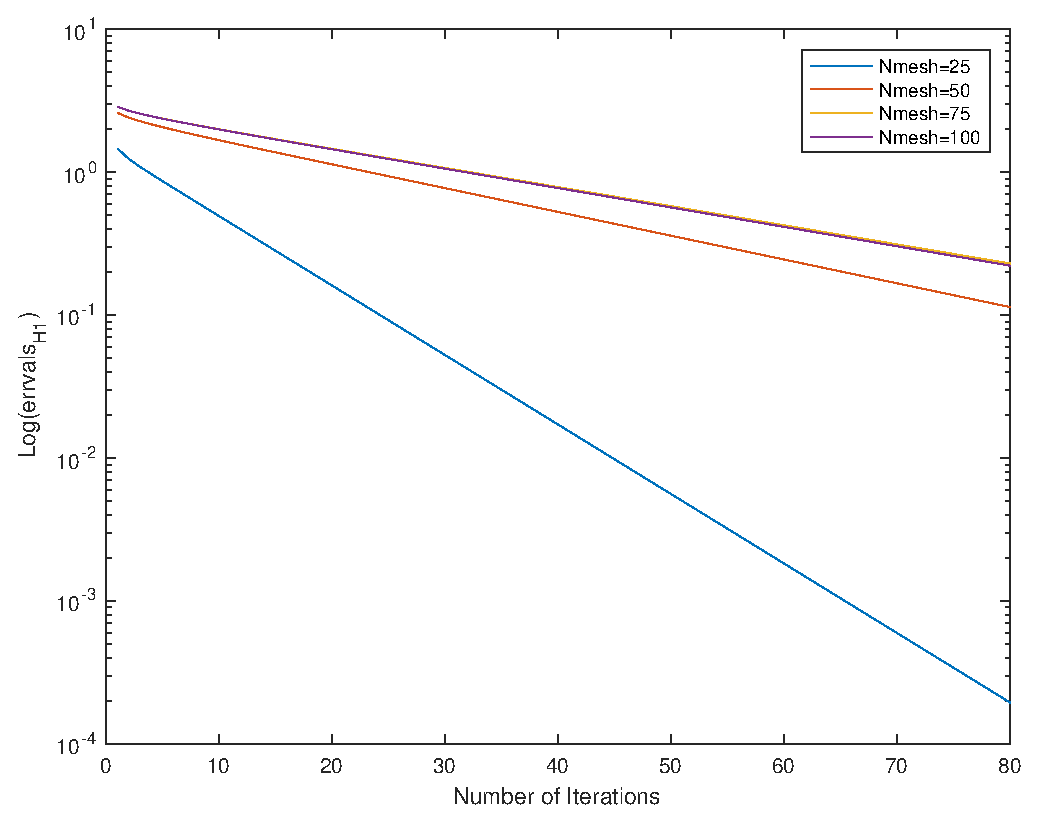
\includegraphics [width=4in]{lshape_neumann_meshsize2_14.eps}


\begin{thebibliography}{10} 
\addtolength{\leftmargin}{0.2in}
\setlength{\itemindent}{-0.2in}
\bibitem[BL97]{BL97} H.H.Bauschke, J.M.Borwein, and A.S.Lewis, \emph{The method of cyclic projections for closed
convex sets in Hilbert space}, Contemporary Mathematics, Vol.204,(1997) 1–38.
\bibitem[BL97]{BL97} H.H.Bauschke, J.M.Borwein, and A.S.Lewis, \emph{The method of cyclic projections for closed
convex sets in Hilbert space}, Contemporary Mathematics, Vol.204,(1997) 1–38.
\bibitem[De83]{De83} F.Deutsch \emph{Applications of von Neumann's alternating projections algorithm}, Mathematical Methods in Operations Research,(1983), 44-51
\bibitem[DH15]{DH15} F.Deutsch, H.Hundal \emph{Arbitrarily slow convergence of sequences of linear operators}, Contemporay Mathematics,Vol. 636,(2015), 93-120
\bibitem[BL97]{BL97} H.H.Bauschke, J.M.Borwein, and A.S.Lewis, \emph{The method of cyclic projections for closed
convex sets in Hilbert space}, Contemporary Mathematics, Vol.204,(1997),1–38.
\bibitem[DH10a]{DH10a}F.Deutsch, H.Hundal \emph{Slow convergence of sequences of linear operators I: Almost
arbitrarily slow convergence}, J.Approx.Theory, 162 (2010),1701-1716.
\bibitem[DH10b]{DH10b}F.Deutsch, H.Hundal \emph{Slow convergence of sequences of linear operators II: Almost
arbitrarily slow convergence}, J.Approx.Theory, 162 (2010),1717-1738.
\bibitem[HS69]{HS69} H.A.Schwarz,\emph{\"{U}ber einige Abbildungsaufgaben} Ges. Math. Abh.,11 (1869), 65-83
\bibitem[IH62]{IH62} I.Halperin, \emph{The product of projection operators}, Acta Sei. Math. (Szeged) 23 (1962) 96-99. 
\bibitem[JN33]{JN33}J. von Neumann \emph{Functional Operators Vol. II. The Geometry of Orthogonal Spaces}, Princeton University Press,Princeton, 1950 (a reprint of mimeographed lecture notes first distributed in 1933). 
\bibitem[KW88]{KW88} S.Kayalar, H.L.Weinert\emph{Error bounds for the method of alternating projects} Math.Control Signals Systems 1(1988) 43-59
\bibitem[NN53]{NN53}N.Nakano \emph{Spectral Theory in the Hilbert Space}, Japan Society for the Promotion of Science, Toyko,1953
\bibitem[NW55]{NW55}N.Wiener, \emph{On the factorization of matrices}, Comment. Math. Helv. 29 (1955) 97-111. 
\bibitem[SK40] {SK40} S.Kakutani, On Nakano's talk, \emph{Zenokuku Sugaku Danwakai Osaka} 192 (1940) 42-44 (Japanese). 
\bibitem[PL88]{PL88} P.L.Lions \emph{On the Schwarz Alternating Method I}, SIAM, Philadelphia, 1988
\end{thebibliography}



\end{document}